%!TEX root = plos_template.tex
% Template for PLoS
% Version 1.0 January 2009
%
% To compile to pdf, run:
% latex plos.template
% bibtex plos.template
% latex plos.template
% latex plos.template
% dvipdf plos.template

\documentclass[10pt]{article}
%\documentclass[aps,twocolumn]{revtex4-1}
%\documentclass[aps,twocolumn]{article}

% amsmath package, useful for mathematical formulas
\usepackage{amsmath}
\setcounter{MaxMatrixCols}{50}
% amssymb package, useful for mathematical symbols
\usepackage{amssymb}

% graphicx package, useful for including eps and pdf graphics
% include graphics with the command \includegraphics
\usepackage{graphicx}

% cite package, to clean up citations in the main text. Do not remove.
\usepackage{cite}

\usepackage{color}

% Use doublespacing - comment out for single spacing
%\usepackage{setspace}
%\doublespacing

% Text layout
\topmargin 0.0cm
\oddsidemargin 0.5cm
\evensidemargin 0.5cm
\textwidth 16cm
\textheight 21cm

% Bold the 'Figure #' in the caption and separate it with a period
% Captions will be left justified
\usepackage[labelfont=bf,labelsep=period,justification=raggedright]{caption}

% Use the Science provided bibtex style
\bibliographystyle{Science}

% Remove brackets from numbering in List of References
\makeatletter
\renewcommand{\@biblabel}[1]{\quad#1.}
\makeatother

% Leave date blank
\date{}

\pagestyle{myheadings}
%% ** EDIT HERE **

\usepackage{bussproofs}

% xy-pic for diagrams
\usepackage[all]{xy}
% subcaption
\usepackage{subcaption}
% hyperref
%\usepackage[linkbordercolor={.67 .27 .27},citebordercolor={.09 .29 .54},urlbordercolor={.09 .29 .54}]{hyperref}
\usepackage{hyperref}
\hypersetup{colorlinks=true,
linkcolor=[rgb]{.67 .27 .27},
citecolor=[rgb]{.09 .29 .54},
urlcolor=[rgb]{.09 .29 .54}}

% color table cells http://goo.gl/ZmpJv
\usepackage[table]{xcolor}
% rotate text in table http://goo.gl/Lb4Zd
\usepackage{rotating}
% listings for code highlighting in appendix
\usepackage{listings}
\usepackage{setspace}
%!TEX root = ../plos_template.tex
% http://widerin.org/blog/syntax-highlighting-for-python-scripts-in-latex-documents
\definecolor{Code}{rgb}{0,0,0}
\definecolor{Decorators}{rgb}{0.5,0.5,0.5}
\definecolor{Numbers}{rgb}{0.5,0,0}
\definecolor{MatchingBrackets}{rgb}{0.25,0.5,0.5}
\definecolor{Keywords}{rgb}{0,0,1}
\definecolor{self}{rgb}{0,0,0}
\definecolor{Strings}{rgb}{0,0.63,0}
\definecolor{Comments}{rgb}{0,0.63,1}
\definecolor{Backquotes}{rgb}{0,0,0}
\definecolor{Classname}{rgb}{0,0,0}
\definecolor{FunctionName}{rgb}{0,0,0}
\definecolor{Operators}{rgb}{0,0,0}
\definecolor{Background}{rgb}{0.98,0.98,0.98}

\lstnewenvironment{python}[1][]{
\lstset{
numbers=left,
numberstyle=\footnotesize,
numbersep=1em,
xleftmargin=1em,
framextopmargin=2em,
framexbottommargin=2em,
showspaces=false,
showtabs=false,
showstringspaces=false,
frame=l,
tabsize=4,
% Basic
basicstyle=\ttfamily\small\setstretch{1},
%basicstyle=\ttfamily\footnotesize,frame=single,#1,
backgroundcolor=\color{Background},
language=Python,
% Comments
commentstyle=\color{Comments}\slshape,
% Strings
stringstyle=\color{Strings},
morecomment=[s][\color{Strings}]{"""}{"""},
morecomment=[s][\color{Strings}]{'''}{'''},
% keywords
morekeywords={import,from,class,def,for,while,if,is,in,elif,else,not,and,or,print,break,continue,return,True,False,None,access,as,,del,except,exec,finally,global,import,lambda,pass,print,raise,try,assert},
keywordstyle={\color{Keywords}\bfseries},
% additional keywords
morekeywords={[2]@invariant},
keywordstyle={[2]\color{Decorators}\slshape},
emph={self},
emphstyle={\color{self}\slshape},
%
}}{}

\usepackage{placeins}

% define colors
\definecolor{DeepRed}{rgb}{.82,.14,.16}
\definecolor{DeepBlue}{rgb}{0,0.36,0.62}

% set depth for table of contents
% http://tex.stackexchange.com/a/17879/6784
% http://tex.stackexchange.com/a/11669/6784
\setcounter{tocdepth}{4}
\setcounter{secnumdepth}{0}

%% ** EDIT HERE **
%% PLEASE INCLUDE ALL MACROS BELOW

% Set autoref text
% http://tex.stackexchange.com/a/36576/6784
\renewcommand*{\figureautorefname}{Fig.}
\renewcommand*{\equationautorefname}{Eq.}
\renewcommand*{\tableautorefname}{Table}

\renewcommand{\refname}{References and Notes}

\newcommand{\beginsupplement}{%
        \setcounter{table}{0}
        \renewcommand{\thetable}{S\arabic{table}}%
        \setcounter{figure}{0}
        \renewcommand{\thefigure}{S\arabic{figure}}%
     }
%% END MACROS SECTION


\begin{document}

% Title must be 150 characters or less
\begin{flushleft}
{\Large
\textbf{Modularization of global genotype-phenotype mappings accesses a relative superset of biological functions}
}
% Insert Author names, affiliations and corresponding author email.
\\
Author1$^{1}$,
Author2$^{2}$,
Author3$^{3,\ast}$
\\
\bf{1} Author1 Dept/Program/Center, Institution Name, City, State, Country
\\
\bf{2} Author2 Dept/Program/Center, Institution Name, City, State, Country
\\
\bf{3} Author3 Dept/Program/Center, Institution Name, City, State, Country
\\
$\ast$ E-mail: Corresponding author@institute.edu
\end{flushleft}

% Please keep the abstract between 250 and 300 words
\section*{Abstract}
%!TEX root = ../plos_template.tex
Different gene regulatory network architectures are commonly thought to provide access to different collections of gene expression patterns that may ultimately result in different phenotypes~\cite{Alon2007}. The manner in which stochasticity in the gene expression process~\cite{Eldar2010,Sanchez2013} impacts the relationship between network architecture and the expression patterns each is capable of producing is not clear~\cite{Jothi2009,Chalancon2012}. In order to investigate this relationship, we begin with the finest grained notion of genotype to phenotype map, gene expression, and adopt a formalism to reason generally about probability distributions over such maps~\cite{Lane1998,MacLane1992,Awodey2006,Abramsky2011}. In all cases, this must be relative to a notion of network architecture, defined here as a hypergraph determining a hierarchical model~\cite{Lauritzen1996} over a given set of genes. We show that in a simple case where the highest-order gene regulatory interactions are allowed, then under some conditions the collection of accessible phenotypes is smaller than in some of the alternative cases in which only lower-order interactions are allowed. This conclusion is arrived at by comparing the geometries of spaces of probability distributions on genotype-phenotype maps for the case of a genome containing a given number of simultaneously interacting genes to the equivalent for all of the other possible gene regulatory network topologies on the same number of genes. We find that the latter spaces of probability distributions associated to the restriction to lower-order interactions are actually larger than the former one whenever the gene regulatory network topology contains a cyclic structure. A generalization of this result to an arbitrary number of genes implies that modularization of interactions, defined here as restriction from relatively higher- to lower-order interactions, within and among gene regulatory networks permits access to additional correlation patterns of expression among multiple interacting genes. That these additional gene expression patterns may enable the fulfillment of functional requirements in certain environments while remaining intrinsically inaccessible when highest-order interactions are allowed implies that, even when gene expression stochasticity is taken into account, network architectures may be functionally differentiated and thus serve as substrate for natural selection in a background of otherwise evolutionarily neutral space. The identification of \emph{interaction constraint}~\cite{Bar-Even2006,Johnson2010a} as an enabler as opposed to a limitation on accessible phenotypes may contribute to a more general explanation for the hierarchical modular architecture~\cite{Ravasz2002,Segre2005,Wagner2007,Erwin2009,Jothi2009,Bhardwaj2010,Colm} of the gene regulatory networks observed throughout the tree of life.


% Please keep the Author Summary between 150 and 200 words
% Use first person. PLoS ONE authors please skip this step.
% Author Summary not valid for PLoS ONE submissions.
\section*{Author Summary}

\section*{Introduction}
%!TEX root = ../plos_template.tex
Probabilistic models of biological networks serve as a bridge between theory and experiment.  On the one hand, parameters in a probabilistic model can be fit to data obtained by measuring the levels of each variable. For example in gene regulatory networks, gene expression can be measured using microarray or sequence census methods \cite{Anastassiou2007,Friedman2008a,Zhang2013}.  On the other hand, one can model a biological network as a deterministic or stochastic reaction network which tracks levels of each molecule \cite{Alon2006,Voit2012}.  From the solution to this latter kind of model, one can then obtain theoretical predictions for the parameters of the probabilistic model in terms of reaction rates.  Comparison of the parameters fitted from data with the predicted values serves as a means for comparing theory with experiment and can serve as a starting point for improving the theory or for designing future experiments \cite{Tonsing2014}.

An important feature of experimental science is that it involves partial information.  In the course of a single measurement, one typically is not able to observe a biological network in its entirety.  Rather, one observes a subnetwork at a time and only obtains a more complete picture by later combining these partial views.  This contrasts with theory, where, one makes a representation of a closed system that provides explicit values for all quantities of interest.  In order for a probabilistic model to serve its purpose, it should also accomodate partial information and thus we will explicitly consider the effects of 1) carving out a subnetwork from its context and 2) coarse-graining observables. Observables representing partial information will generally arise in situations where a system is interacting with another system. This situation arises in the context of interpreting the potential existence of modular substructure within biological network data deriving from any given organism as well as with respect to the interactions between an organism and its environment.

% Studying this situation, we find that instances arise where the fact that a network context may interact with only partial information of the states of a given subnetwork can result in apparent inconsistency. Furthermore,

Inconsistency arises when a network context places more constraints on a subnetwork than it is capable of satisfying. The impact of this issue on genetic interactions has been considered previously in the context of population genetics \cite{EthanAkin389}. We exhibit a method of checking for such consistency and evaluating its likelihood of arising in the context of building probabilistic models of biological networks. When apparent inconsistency is observed, it must arise from the network context interacting with only partial information of the states of a given subnetwork. This would indicate that information about the network context must be included in order to maintain a consistent model of the system.

% Consider the case in which the network context is an environment placing independent and identical functional requirements upon a population of similar independent subnetworks and selecting for their architectures over many generations to satisfy those requirements. Our analysis of the probability of inconsistency arising relative to network architecture demonstrates that networks with a larger number of cycles are more likely to be subjected to inconsistent constraints that will be unable to be jointly satisfied. Since this probability of inconsistency is higher for networks with a larger number of cycles, this results in implicit selection against biological network architectures with a larger number of cycles. One would not expect such a bias to eliminate the existence of cycles in biological networks. However, it is reasonable to expect on the basis of this result a kind of hierarchical modularity: where modules that may possess cycles and are small relative to the overall size of the network exist within a globally hierarchical network structure. A similar problem has been considered previously in the context of population genetics \cite{EthanAkin389}. Of course, there are other factors which may contribute to the development of such network architectures. The evaluation of the hierarchical modularity property will require extensive future work, but its existence is consistent with many studies that have evaluated the architecture of various biological networks~\cite{Ravasz2002,Segre2005,Wagner2007,Erwin2009,Jothi2009,Bhardwaj2010,Chalancon2012,Colm}.

In \ref{sec:networkcontext} we describe the relationship between representations of biological networks and an abstraction of these referred to as network architecture that indicates the manner in which a subset of a network is connected to its context. We explain the connection between stochastic process models of biological networks and a generalization of the genotype-phenotype map applying to arbitrary biological networks referred to as \gnpm{} in \ref{sec:genenetworkphenmap}. \ref{sec:probabilitydistributionsonnetworks}--\ref{sec:inconsistency} contain examples of the underlying mathematical justification for our claims (more details of which are provided in \refsupp{}), and they can be skipped by readers who are primarily interested in the intuitive implications of our analysis. In \ref{sec:probabilitydistributionsonnetworks} we introduce the concept of network modules and define probability distributions over their states. \ref{sec:compatibilityofgpms} and \ref{sec:inconsistency} describe the different compatibility conditions that arise for different biological network architectures and demonstrate how these compatibility conditions lead to a set of inequalities determining a space of probability distributions for each network architecture. \ref{sec:cycliccontextunsatisfiableconstraints} and \ref{sec:probconstrgeometry} examine these constraints for the example of the three-cycle network architecture. \ref{sec:volrat} computes the likelihood of unsatisfiable constraints for all biological network architectures on four variables that possess cycles. Finally, \ref{sec:unsatisfiableconstrevolution} explains implications for the evolution of biological network architectures of the result that networks with a larger number of cycles are more likely to have unsatisfiable constraints placed upon them.

% We explain how one can pass from relatively fine-grained to more coarse-grained descriptions such as the ability to produce a given metabolite in a manner that is dependent upon interactions among multiple genes in \ref{secsupp:coarsegrainingphenotypes}. In \ref{sec:covergenotypespace} we define a biological network architecture as a collection of subsets of variables that together comprise a larger set. The different ways in which this is accomplished correspond to distinct BNAs.

% Traditional dynamical models of gene-regulatory networks begin by treating them as reaction networks whose known or hypothesized interactions are encoded by sigmoidal response functions \cite{Alon2006,Voit2012}. Genes that interact do so in such a manner as to either activate or inhibit one another leading to a dynamical model of the gene expression process.
% \begin{eqnarray*}
% {dg_i \over dt} =
% k_{is}  \prod_{j=1}^{N} \frac{k_{ija} g_j^{n_{ija}}}{1+k_{ija} g_j^{n_{ija}}}
% \frac{1}{1+k_{ijr} g_j^{n_{ijr}}} - k_{id} g_i
% \end{eqnarray*}
% for a network of $N$ genes where $g_i$s represent concentrations of gene products, $k_{ija}$s represent activation rates, $k_{ijr}$s represent repression rates, and $k_{id}$s represent degradation rates.
% The dual perspective is taken by probabilistic models whose parameters are fit to data obtained by measuring gene expression using microarray or sequence census methods \cite{Friedman2008a,Zhang2013}.
% In both of these classes of models, higher-order correlations are assumed to be accurately represented in terms of a sum over lower-order correlations.

% The evolution of \gnpm{} is an open question in biology. Specifically, how the higher level constraints imposed upon a system at a phenotypic level shape the elements and the interaction among the elements at a lower, genotypic level. Here we neglect the specific mechanisms by which one achieves such phenotypes and assume a statistical view of the observed phenotype. This communication introduces a framework that enable us to analyze how higher-level constraints, formulated in terms of probability of gene expression pattern might shape the allowable interactions among elements at a lower level.

% The genotype of an organism has a relatively straightforward definition in terms of the sequence of nucleotides comprising its genome. Phenotypes, on the other hand, can be described at different levels of organization~\cite{Dawkins1982,Stadler2001}. The concept of phenotype was initially defined at the level of macroscopically observable physical characteristics such as shape, size, color, and various combinations thereof~\cite{Johannsen1911}. However, since the advent of molecular biology, the lowest level description of phenotype might be considered to be the dynamic phenomenon that can be described by measuring the transcription states of all genes comprising an organism's genome. The time series that results from such observations can be used to infer various statistics that characterize gene expression such as correlations between pairs of genes. The statistics associated to any higher-level phenotype that is determined by a particular gene expression pattern should be functions of such statistics.

% % The present capability to observe phenotypes at various levels of organization raises several questions about \gnpm{}. One is how to define and characterize properties of the fundamental level of \gnpm{} that is embodied in the transcription process. Another is how to define and characterize the manner in which higher-order ``phenotype$_i$-phenotype$_{i+1}$'' mappings built on top of this one are affected by the properties of each of the levels existing below, and, on evolutionary timescales over which feedback may play a significant role, potentially also those above it.

% % We attempt to address these questions from an abstract perspective that is independent of the particular physical implementation of \gnpm{} in terms of complex networks of molecular interactions.
% We present a formal probabilistic description of the \gnpm{} that takes into account higher-order correlations among genes as well as evidence that gene expression is stochastic \cite{Swain2002,Paulsson2004,Thattai2004,Acar2008a,Lestas2010,So2011,Munsky2012,Neuert2013,Sanchez2013}. In order to assess the impact of these features on the evolution of gene regulatory network architecture, where architecture is here considered to be determined exclusively by observable correlations among genes \cite{Friedman2008a}, we use this description to precisely pose the question: For any genotype, given a space of probability distributions on the collection of \gnpm{}, does modularization of the genotype (restriction of correlations among genes, \refsupp{}) increase, decrease, or leave invariant the size of the accessible space of selectable gene expression patterns?
% % For example, if we have three genes that can all participate in a higher-order interaction (the highest-order among three genes being a trinary interaction) that generates a phenotype, but we restrict interactions to a lower-order subset consisting of all three possible binary interactions then this represents one particular way of modularizing over a given genotype (compare \ref{fig:conediagram}B top and middle).

% For those cases in which modularization results in no change to the space of probability distributions over \gnpm{} with respect to that defined on the full genotype (i.e. the single highest-order correlation referred to as non-modular), then there may be no method to select for one network architecture over another. On the other hand any differences in gene expression patterns that result from differences in network architecture may allow certain network architectures to be selected relative to one another. Here we show that those modularizations that introduce cycles into the gene-regulatory network architecture also expose the capacity for negative selection as a result of additional restrictions upon the gene expression patterns that apply to networks with cycles but not to those without.

% % then there would be no way to observationally distinguish the collection of possible gene expression patterns of organisms incorporating molecular mechanisms that explicitly impose such modularity, and thus no means of selecting specifically for modular or non-modular gene regulatory networks~\cite{Jothi2009,Colm}. If, on the other hand, modularization provides access to a larger or smaller space of probability distributions over \gnpm{} than for the non-modular case, then one can imagine that certain environmental conditions would be unable to be addressed by the functions capable of being achieved by the gene expression profiles accessible to one gene-regulatory network with respect to another. We provide a precise quantitative answer to the question stated above for several different modularizations over a collection of interacting genes.

% % In a network context in which all interaction orders are allowed, restriction of higher-order interactions within the underlying process intuitively reduces the size of the space of accessible gene expression patterns. However, in network contexts that are constrained to match the stationary structure of the underlying process, modularizations over a genotype that include at least one cycle in the hypergraph representing the resulting modular structure provide access to a \emph{larger} collection of potential gene expression patterns and thus a larger collection of potential biological functions that may derive from the expanded repertoire of such patterns. We provide a precise quantitative answer to the question stated above for several different modularizations over a collection of interacting genes.



% Results and Discussion can be combined.
\section*{Model description}

\subsection*{Deterministic genotype-phenotype maps}
Consider the case in which we have an arbitrary number of \emph{genes} indexed by $i=1, \ldots, m$. There is a particular set of potential \emph{genes} denoted $L$. A subset of genes will be denoted as $U \subseteq L$. We also have a set of phenotypes $P$. In principle, any gene could give rise to any phenotype. A genotype-phenotype map is thus represented as a function mapping a subset of genes into phenotypes
$$
e \colon U \rightarrow  P.
$$

In the observationalist framework from which this modeling description derives \cite{Abramsky2011}, our genes $L$ are analogous to measurements $T \subseteq X$ and our phenotypes $P$ are like measurement outcomes or values $V$. An event in which outcomes $s(t)$ are observed for each $t \in T$ serve to define mappings called \emph{sections} over $T$ as

$$
s \colon T \rightarrow V.
$$

We denote the set of all subsets of a set $X$ as $\mathcal{P}(X)$. $\mathcal{P}(L)$ can then be viewed as a category in which the objects are subsets of genes and morphisms represent inclusion of a smaller subset into a larger superset (i.e. $U \subseteq U' \Rightarrow U \rightarrow U'$). The category $\mathcal{P}(L)^{opp}$ then has the same objects, but the morphisms represent restriction from a larger to a smaller subset of alleles (i.e. $U' \supseteq U \Rightarrow U' \rightarrow U$). In order to consider the set of all genotype-phenotype maps together, we can construct a functor
$$
\mathcal{E} \colon \mathcal{P}(L)^{opp} \rightarrow Set
$$
by exhibiting precisely how it acts on objects and morphisms in its domain category. We explicitly represent the way in which the functor $\mathcal{E}$ acts on objects and morphisms $U$ and $U \subseteq U'$ respectively as
\begin{equation}\label{eq:gpfunctor}
\begin{split}
\mathcal{E} \colon \mathcal{P}(L)^{opp} &\rightarrow Set,\\
U &\mapsto P^U,\\
U \subseteq U' &\mapsto res^{U'}_{U}.
\end{split}
\end{equation}
So the functor $\mathcal{E}$ takes a subset of genes and returns the set of genotype-phenotype mappings from the given subset of genes to the set of phenotypes. The restriction map operates on sets deriving from the application of $\mathcal{E}$ to a subset of genes as follows
\begin{eqnarray*}
res^{U'}_{U} \colon \mathcal{E}(U') &\rightarrow& \mathcal{E}(U)\\
P^{U'} &\rightarrow& P^U\\
e' \colon U' \rightarrow P &\mapsto& e'|_U \colon U \rightarrow P
\end{eqnarray*}
$\mathcal{E}$ is thus, by definition, a presheaf functor, which is an object in the functor category $Sets^{\mathcal{P}(L)^{opp}}$.

\subsection*{Stochasticity among genotype-phenotype maps}
There may be several sources for stochasticity in genotype-phenotype mapping including small numbers of the causal molecules and products of gene expression as well as environmental fluctuations upon which genotype-phenotype mappings are conditioned \cite{Swain2002,Paulsson2004,Thattai2004,Acar2008a,Lestas2010,Munsky2012,Neuert2013}. Here we generalize the deterministic framework outlined above to the stochastic case.

An \emph{algebraic structure} is determined by a set and one or more finitary operations (e.g. binary multiplication) defined on the elements of that set. A \emph{monoid} is a type of algebraic structure determined by a set and a binary operation such that the latter satisfies closure, associativity and identity with respect to the given set. A \emph{semiring} is an algebraic structure determined by a set with two binary operations. One of the binary operations, addition, forms a commutative monoid and has identity element 0. The second binary operation, multiplication, is a monoid with identity element 1. These binary operations interact such that multiplication distributes over addition and multiplication by the identity element of the addition monoid annihilates all elements in the semiring. For example, the real numbers under addition and multiplication constitute a semiring whose data is described as $\left( \mathbb{R},+,0,\times,1 \right)$.

Consider a function, $\phi$ from a set, $L$, to a semiring $R$ written $\phi \colon L \rightarrow R$. The \emph{support} of $\phi$, $\text{supp}(\phi)$, is then the set $\{ l \in L | \phi(l) \neq 0 \}$. A distribution with respect to the semiring $R$ on $L$ is given as a function having finite support and satisfying a constraint
\begin{eqnarray*}
d \colon L \rightarrow R,\\
\sum_{l \in L} d(l) = 1
\end{eqnarray*}
We can consider the set of all distributions with respect to a given semiring $R$ satisfying the above constraints and defined on the set $L$ as being given by a functor applied to $L$ as $\mathcal{D}_R (L)$. We can again explicitly represent the way in which the functor $\mathcal{D}_R$ acts on objects and morphisms $L$ and $f \colon L \rightarrow M$ as
\begin{equation}\label{eq:distfunctor}
\begin{split}
\mathcal{D}_R \colon Set &\rightarrow Set,\\
L &\mapsto \mathcal{D}_R (L),\\
f \colon L \rightarrow M &\mapsto \mathcal{D}_R (f) \colon \mathcal{D}_R (L) \rightarrow \mathcal{D}_R (M),
\end{split}
\end{equation}
where
\begin{eqnarray*}
\mathcal{D}_R (f) \colon \mathcal{D}_R (L) &\rightarrow& \mathcal{D}_R (M),\\
d &\mapsto& \left[ m \mapsto \sum_{f(l)=m} d(l) \right].
\end{eqnarray*}
For the case in which we consider $R$ to be the semiring of non-negative real numbers $\left( \mathbb{R}_{\geq 0},+,0,\times,1 \right)$, $\mathcal{D}_R (L)$ represents the set of probability distributions on the set $L$.

Recalling the presheaf functor, $\mathcal{E} \colon \mathcal{P}(L)^{opp} \rightarrow Set$, mapping genotypes to the set of maps from those genotypes to the set of phenotypes, we can now compose it with the distribution functor $\mathcal{D}_R$ to obtain a new presheaf functor $\mathcal{D}_R \circ \mathcal{E} \colon \mathcal{P}(L)^{opp} \rightarrow Set \rightarrow Set$ that assigns to each genotype a distribution over the set of maps from those genotypes to the set of possible phenotypes. The action of $\mathcal{D}_R \mathcal{E}$ on objects and morphisms in $\mathcal{P}(L)^{opp}$ yields
\begin{eqnarray*}
\mathcal{D}_R \mathcal{E} \colon \mathcal{P}(L)^{opp} &\rightarrow& Set,\\
U &\mapsto& \mathcal{D}_R \mathcal{E}(U) \equiv d \colon P^U \rightarrow R,\\
U \subseteq U' &\mapsto& \mathcal{D}_R \mathcal{E}(U') \rightarrow \mathcal{D}_R \mathcal{E}(U).
\end{eqnarray*}
where
\begin{eqnarray*}
\mathcal{D}_R \mathcal{E}(U') &\rightarrow& \mathcal{D}_R \mathcal{E}(U),\\
d \colon P^{U'} \rightarrow R &\rightarrow& d|U \colon P^{U} \rightarrow R
\end{eqnarray*}
and
\begin{eqnarray*}
d \colon P^{U'} &\rightarrow& R,\\
s' &\mapsto& d(s');\\
d|U \colon P^{U} &\rightarrow& R,\\
s &\mapsto& \sum_{s' \in \mathcal{E}(U'),\, s'|U=s} d(s').
\end{eqnarray*}

\subsection*{Coverings of genotype space}
A \emph{gene regulatory network module} is represented by a tuple of genes $O$ and a collection of gene regulatory network modules, which in some cases may represent all of the genes in an organism, is a set of such tuples $\mathcal{G}$ (i.e. $O \in \mathcal{G}$). An individual may be composed of some collection of subsets of possible genes where the set of all genes, $L$, is viewed as the genotype space. A \emph{covering} of the genotype space, $\mathcal{G}$, satisfies $\cup_i \mathcal{G}_i = L$ and $O,O' \in \mathcal{G}$ and $O \subseteq O'$ means that $O = O'$. The first condition means that $\mathcal{G}$ covers $L$ and the second conditions means that if a given subset of genes $O'$ is compatible in a sense to be explained more precisely in what proceeds then any smaller subset of genes $O$ is also compatible.

\subsection*{Compatibility of distributions on genotype-phenotype maps}
Given a covering of the genotype space $\mathcal{G}$, a compatible family for $\mathcal{G}$ with respect to the distribution presheaf $\mathcal{D}_R\mathcal{E}$ is given by a family of distributions $\{d_O \colon P^O \rightarrow R | O \in \mathcal{G}\}$ such that
\begin{eqnarray*}
\forall O \in \mathcal{G} \left[ \exists d_O \in \mathcal{D}_R\mathcal{E}(O) \right],\\
d_O|O \cap O' = d_{O'}|O \cap O'.
\end{eqnarray*}
The second condition, $d_O|O \cap O' = d_{O'}|O \cap O'$, is referred to as the \emph{sheaf condition}. This condition means that any two distributions $d_O$ and $d_{O'}$ in the \emph{compatible family} of distributions produce the same values in the semiring $R$ on all of the genes in the intersection of $O$ with $O'$.

For example, if we have two gene regulatory network modules given by their genotypes $O = \{l_1, l_2\}$ and $O' = \{l_1, l'_2\}$ then the sheaf condition specifies that for $e_{\{l_1\}} \in \mathcal{E}(\{l_1\})$, which assigns a particular phenotype to the genotype $\{l_1\}$, that
\begin{eqnarray}\label{eq:sheafprob}
\sum_{e \in \mathcal{E}(O),\, e|l_1=e_{\{l_1\}}} d_O(e) \,\, = \sum_{e' \in \mathcal{E}(O'),\, e'|l_1=e_{\{l_1\}}} d_{O'}(e')
\end{eqnarray}
This condition means that the probability for gene $i=1$ to be associated to the phenotype given by $e_{\{l_1\}}$ is equivalent in case we marginalize over either possible \emph{allele} for gene $i=2$.

\subsection*{Global sections of distributions over genotype-phenotype maps}
To say that the sheaf condition holds for a compatible family $\{d_O\}_{O \in \mathcal{G}}$ for the presheaf $\mathcal{D}_R\mathcal{E}$ implies the existence of a \emph{global section} $d \in \mathcal{D}_R\mathcal{E}(L)$ that is defined on the full set of genes. An example of a distribution that could be a global section given that it satisfies the sheaf condition is shown in Table \ref{tab:hidvarmod}. This global section defines a distribution on the set of genotype-phenotype maps given by $\mathcal{E}(L) = P^L$, specifying phenotypes associated to all genes at once instead of on subsets of $L$ associated to either $U \subseteq L$ or, what is essentially equivalent, $O \in \mathcal{G}$. Crucially, the distribution $d$ must also restrict for the subset of genes associated to any gene regulatory network module, which in some cases may represent all of the genes in an organism, $O$ in a covering of the genotype space $\mathcal{G}$ meaning that
\begin{eqnarray}
\forall O \in \mathcal{G} \left[ d|O = d_O \right].
\end{eqnarray}
In terms of distributions, the existence of a global section $d$ for a covering of the genotype space $\mathcal{G}$ corresponds to the existence of a distribution defined on all genes that marginalizes to yield the distributions on subsets of genes that may be observed empirically.

The presheaf $\mathcal{E}$ alone was already a sheaf because given a cover $\{U_i\}_{i \in I}$ of $U$ there is a family of sections $\{e_i \in \mathcal{E}(U_i)\}_{i \in I}$ that is compatible in the sense that
\begin{eqnarray}
\forall i,j \in I \left[ e_i|U_i \cap U_j = e_j|U_i \cap U_j \right].
\end{eqnarray}
In this case there is a unique global section $e \in \mathcal{E}(U)$ such that $\forall i \in I \left[ e|U_i = e_i \right]$. The fact that the sheaf condition holds for $\mathcal{E}$ is true because we are considering functions defined on a space with a trivial discrete topology allowing us to combine any partial functions that agree on overlapping subsets by taking the union of the data defining such functions.

Extending this example on an arbitrary subset $U \subseteq L$ to the whole set of genes $L$ we have a unique global section $e \in \mathcal{E}(L) = P^L$. $e$ can be used to deterministically assign phenotypes to the set of genes $L$ under consideration.

\subsection*{Example}
We can begin to construct an example to make the model description, so far, more concrete. For this example, we take the full set of potential genes to be $L = \{ l_1,l'_1,l_2,l'_2 \}$. Consider the case in which each of the gene regulatory network modules under consideration each has two genetic loci, $L_1$ and $L_2$, each of which is capable of containing one of two different alleles: $l_1$ or $l'_1$ for $L_1$ and $l_2$ or $l'_2$ for $L_2$. Then we have a covering of the genotype space given by $\mathcal{G} = \{\{l_1,l_2 \},\{l_1,l'_2 \},\{l'_1,l_2\},\{l'_1,l'_2\} \}$. We also have two phenotype values $P = \{0, 1\}$. Each genotype-phenotype map in Table \ref{tab:gpm} assigns phenotype values to each $O \in \mathcal{G}$. For example, $e_1 \colon	l_1 l_2 \rightarrow 00$. Table \ref{tab:probabilities} likewise assigns probabilities to each of these genotype-phenotype mappings.

We can collect all of these genotype-phenotype mappings into one set using the functor given in Equation \ref{eq:gpfunctor} as $\mathcal{E}(\mathcal{G}) = P^{\mathcal{G}} = \{e_i | i=1 \ldots 16 \}$. We may further apply the $R$-distribution functor $\mathcal{D}_R$ given in Equation \ref{eq:distfunctor} to obtain a distribution on the genotype-phenotype mappings. Doing so yields  $\mathcal{D}_R\mathcal{E}(\mathcal{G})=d \colon P^\mathcal{G} \rightarrow R$. If we now apply this distribution function $d$ to the set of genotype-phenotype mappings we get the probabilities associated to each genotype-phenotype map $d(\{e_i | i=1 \ldots 16 \}) = \{p_i|i=1 \ldots 16\}$ given in Table \ref{tab:probabilities}. This can also be written more abstractly as $\left[\mathcal{D}_R\mathcal{E}(\mathcal{G})\right](\{e_i | i=1 \ldots 16 \}) = \left[\mathcal{D}_R\mathcal{E}(\mathcal{G})\right](P^\mathcal{G}) = \left[\mathcal{D}_R\mathcal{E}(\mathcal{G})\right](\mathcal{E}(\mathcal{G})) = \{p_i|i=1 \ldots 16\}$. Notice that we applied the functors $\mathcal{E}$ and $\mathcal{D}_R$ to a specific set, which was all of $\mathcal{G}$. We could have applied these functors to any $O \in \mathcal{G}$. In one case, for example if we take $O = \{l_1, l_2\}$, we would have gotten $\mathcal{E}(O) = \{e_i|i=1 \ldots 4\}$ and $\mathcal{D}_R\mathcal{E}(O) = d \colon P^O \rightarrow R$. In this case $\left[\mathcal{D}_R\mathcal{E}(O)\right](\mathcal{E}(O)) = \{p_i|i=1 \ldots 4\}$.

We may also consider directly the meaning of $\left[\mathcal{D}_R\mathcal{E}(\{l_1\})\right](\mathcal{E}(\{l_1\}))$ and similarly for the other $l \in L$. The sheaf condition then introduces a system of equations relating and thus constraining the probability parameters, beyond the constraint that each row sum to one. The constraint introduced by the sheaf condition is expressed in Equation \ref{eq:sheafprob}, specialized to this example by
\begin{eqnarray}\label{eq:sheafprob2}
\sum_{e \in \mathcal{E}(\{l\}),\, e|l=e_{\{l\}}} d_{\{l\}}(e) \,\, = \sum_{e \in \mathcal{E}(O),\, e|l=e_{\{l\}}} d_O(e) \,\, = \sum_{e' \in \mathcal{E}(O'),\, e'|l=e_{\{l\}}} d_{O'}(e'),
\end{eqnarray}
for each $l \in L$, $e_{\{l\}} \in \mathcal{E}(\{l\})$, and $\{O \in \mathcal{G}|l=o, o \in O\}$. The resulting equations are explicitly indicated in like colors between the columns of Table \ref{tab:sheaf} :
\begin{equation}
\begin{aligned}\label{eq:pparsys}
p^*_1 &= p_1 + p_3 = p_5 + p_7, &
p^*_2 &= p_2 + p_4 = p_6 + p_8,\\
p^*_3 &= p_9 + p_{11} = p_{13} + p_{15},&
p^*_4 &= p_{10} + p_{12} = p_{14} + p_{16},\\
p^*_5 &= p_1 + p_2 = p_9 + p_{10},&
p^*_6 &= p_3 + p_4 = p_{11} + p_{12},\\
p^*_7 &= p_5 + p_6 = p_{13} + p_{14},&
p^*_8 &= p_7 + p_8 = p_{15} + p_{16}.
\end{aligned}
\end{equation}

Consider the meaning of the sheaf condition for $\mathcal{D}_R\mathcal{E}(L)$. $d \in \mathcal{D}_R\mathcal{E}(L)$ specifies a distribution whose domain consists of deterministic functions $\mathcal{E}(L) = P^L$ that map each gene independently, and independent of the fact that some combinations of genes  comprise gene regulatory network modules consisting of potentially interacting genes, to a phenotype. Since we have stated that $\mathcal{E}(L)$ satisfies the sheaf condition, for a given covering of the genotype space, $\mathcal{G}$, a globally compatible function $e \in  \mathcal{E}(L)$ restricts to $e|O$ for each $O \in \mathcal{G}$ such that there is a tuple of phenotypes assigned to genes that participate in overlapping gene regulatory network modules. Each $e \in P^L$ is associated to a trivial distribution $\delta_e \in \mathcal{D}_R\mathcal{E}(L)$ such that
\begin{eqnarray}
\delta_e(e') =
\begin{cases}
1, & e' = e,\\
0, & e' \neq e.
\end{cases}
\end{eqnarray}
For each gene regulatory network module $O$ we note that $\delta_e|O = \delta_{e|O}$. In this case, we can write the empirically determined distribution such as Table \ref{tab:probabilities} for a particular gene regulatory network module $d_O$ in terms of the distribution defined on the global set of genes restricted to a particular gene regulatory network module $d|O$:
\begin{equation}\label{eq:factordist}
\begin{split}
d_O(e) &= d|O(e)\\
&= \sum_{e' \in \mathcal{E}(L),e'|O=e} d(e')\\
&= \sum_{e' \in \mathcal{E}(L)} \delta_{e'|O}(e) \times d(e') = \sum_{e' \in \mathcal{E}(L)} \delta_{e'}|O(e) \times d(e')
\end{split}
\end{equation}
where
\begin{equation*}
\delta_{e'}|O(e) = \prod_{o \in O} \delta_{e'|\{o\}}(e|\{o\}).
\end{equation*}
We recover the empirically determined distribution as a sum over the deterministic genotype-phenotype mappings weighted by the probabilities of the distribution $d \in \mathcal{D}_R\mathcal{E}(L)$ defined over the full set of such deterministic mappings.

Thus, when there is a global section, given by $d \in \mathcal{D}_R\mathcal{E}(L)$, for an empirically determined distribution on genotype-phenotype mappings, for example that in Table \ref{tab:probabilities}, then it may be the case that a mechanism that stochastically selects among deterministic genotype-phenotype maps can satisfy or generate an empirically determined distribution.

\subsection*{Existence of a global section for an empirically determined distribution of genotype-phenotype mappings}
Given an empirically determined distribution on the genotype-phenotype mapping process, it may be helpful to be able to classify whether or not there exists a global section satisfying the sheaf condition in order to determine the modularity requirements of the empirical distribution. If an empirically determined distribution does have a global section, then it is possible to achieve the same global biological function specified in the empirical distribution using a single gene regulatory network module that contains all of the genes in the given universal set of genes $L$ as is obtained using the particular cover of the genotype space $\mathcal{G}$ that is associated to the empirically determined distribution. If the empirically determined distribution does not have a global section satisfying the sheaf condition, then there is some contingency regarding interactions between genes necessitating decomposition into smaller submodules than is represented by the whole of the universal set of genes $L$.

For a cover of the genotype space, $\mathcal{G}$, we can construct an incidence matrix, $\mathbf{G}$, representing the relationship between genotype-phenotype mappings having as domain particular gene regulatory network module contexts given by the $O \in \mathcal{G}$ and those global genotype-phenotype mappings defined on $L$. This is equivalent to the more formal statement that there is some binary relation,
\begin{equation}
R \subseteq \mathcal{E}(L) \times \coprod_{O \in \mathcal{G}} \mathcal{E}(O),
\end{equation}
whose \href{http://en.wikipedia.org/wiki/Logical_matrix#Matrix_representation_of_a_relation}{logical matrix representation}, $\mathbf{G}$, we would like to construct. In the first case, $\mathcal{E}(L) = P^L$ we have $\{t_1, \ldots t_m\} = \{t_j | t_j \in P^L\}$. In the second case, $\coprod_{O \in \mathcal{G}} \mathcal{E}(O)$, we have $\{e_1, \ldots e_n\} = \coprod_{O \in \mathcal{G}} \mathcal{E}(O)$. So we have two sets of maps, one defined on $P^L$ and the other defined on $\mathcal{E}(O) = P^O$ for each $O \in \mathcal{G}$. This yields a method of specifying the intended relationship that defines $\mathbf{G}_{n \times m}$ in terms of $t_j \in P^L$ and $e_i \in \mathcal{E}(O)$ :
\begin{eqnarray}
\mathbf{G}[i,j] =
\begin{cases}
1, & t_j|O = e_i,\\
0, & \text{otherwise}.
\end{cases}
\end{eqnarray}
This matrix can be viewed as an operator acting via matrix multiplication on distributions
\begin{eqnarray*}
\mathbf{G} \colon \mathcal{D}_R\mathcal{E}(L) &\rightarrow& \mathcal{D}_R\mathcal{E}(\mathcal{G}),\\
d &\mapsto& (d|O)_{O \in \mathcal{G}},
\end{eqnarray*}
and thereby taking a global distribution defined on genotype-phenotype maps whose domain is the full set of genes $L$ to the \emph{marginalized} distributions that are defined relative to gene regulatory network modules contained in a covering of the genotype space $\mathcal{G}$. This is to say that $\mathbf{G} \cdot d = (d|O)_{O \in \mathcal{G}} = \{d_O\}_{O \in \mathcal{G}}$. $\mathbf{G}$ provides a way of determining the kinds of environmentally determined distributions on genotype-phenotype mapping (i.e. $\{d_O\}_{O \in \mathcal{G}}$, Table \ref{tab:probabilities}) that can be derived from distributions (i.e. $\mathcal{D}_R \mathcal{E}(L)$) defined on the global genotype-phenotype mappings (i.e. $\mathcal{E}(L)$ as opposed to $\mathcal{E}(O)$).

If we have an experimentally determined distribution on genotype phenotype maps in different genetic contexts (e.g. in Table \ref{tab:probabilities}) that we refer to as $\{d_O\}_{O \in \mathcal{G}}$, then we have an assignment of a probability value in $R$ to each genotype phenotype map $e_i \in \mathcal{E}(O)$ in Table \ref{tab:gpm}. We can collect these probabilities into a vector $\mathbf{V}_{n \times 1}$ where we note that $n$ is the same as that used to specify the number of genotype-phenotype maps in the coproduct over gene regulatory network modules in a given covering of the genotype space $\{e_1, \ldots e_n\} = \coprod_{O \in \mathcal{G}} \mathcal{E}(O)$. We can specify as unknown a distribution on the set of globally defined genotype phenotype maps and collect the associated probabilities in a vector $\mathbf{X}_{m \times 1}$ where there is a probability weight associated to each $t_j \in \mathcal{E}(L)$. Now we can attempt to determine the probability distribution on globally defined genotype-phenotype mappings $\mathcal{E}(L)$ by solving the linear system of equations
\begin{equation}
\begin{split}
\mathbf{G}_{n \times m} \mathbf{X}_{m \times 1} = \mathbf{V}_{n \times 1},\\
\sum_{i=1}^{m} \mathbf{X}_{i} = 1.
\end{split}
\end{equation}
The constraint that $\mathbf{X}$ sum to one in order to satisfy the definition of a probability distribution can be integrated into the matrix equation by adjoining a row containing ones to $\mathbf{G}_{n \times m}$ and a row containing a one to $\mathbf{V}_{n \times 1}$
\begin{equation}\label{eq:auglinsys}
\mathbf{G}_{(n + 1) \times m} \mathbf{X}_{m \times 1} = \mathbf{V}_{(n + 1) \times 1}.
\end{equation}
Solutions, if any, to Equation \ref{eq:auglinsys} serve to exhibit a global section for the empirically determined distribution specified in $\mathbf{V}$.

\subsection*{Example global section determination}
There are three parameters that determine the relative size of important sets for understanding the model at hand. $g$ represents the number of genetic loci, $a$ represents the number of different alleles that can occur at each locus, and $p$ represents the number of different phenotype values that each locus can take on. From these parameters, which we use together to classify models satisfying the structural constraints described thus far, we can derive additional quantities characterizing the model. For a system with parameters $(g,a,p)$ there are $a^g$ different gene regulatory network modules to consider and each may be associated with $p^g$ phenotypes. There are thus $(ap)^g$ different genotype-phenotype maps to consider with respect to the gene regulatory network modules meaning that this is the size of the set $\coprod_{O \in \mathcal{G}} \mathcal{E}(O)$. The set of all possible genes $L$ has size $ga$ and since there are $p$ different phenotypes that each gene can be mapped to, there are $p^{ga}$ different globally defined genotype-phenotype maps meaning that this is the size of the set $\mathcal{E}(L) = P^L$. Now we can state the size of the sets $\{t_1, \ldots t_m\} = \{t_j | t_j \in P^L\}$ and $\{e_1, \ldots e_n\} = \coprod_{O \in \mathcal{G}} \mathcal{E}(O)$ because we have explicit formulas for $n = (ap)^g$ and $m = p^{ga}$ in terms of the defining characteristics of a $(g,a,p)$ class of models. From the values of $n$ and $m$ we know the dimensions of the logical matrix representation of the relation $R$ as $\mathbf{G}_{(ap)^g \times p^{ga}}$.

For the case $(g=2,a=2,p=2)$, Table \ref{tab:pars222} shows the relationship between the abstract notation used throughout the model description and the concrete parameters introduced in this example. Using the notation of Table \ref{tab:pars222}, we can also explicitly construct $\mathbf{G}_{(ap)^g \times p^{ga}}$ as in Table \ref{tab:logmat222}.

In terms of the probability values expressed in tables \ref{tab:hidvarmod} and \ref{tab:probabilities} the resulting system of equations $\mathbf{G}_{n \times m} \mathbf{X}_{m \times 1} = \mathbf{V}_{n \times 1}$ is
\begin{equation}
\begin{aligned}\label{eq:globsys}
p_1 &= q_1 + q_2 + q_3 + q_4 &
p_2 &= q_5 + q_6 + q_7 + q_8 \\
p_3 &= q_9 + q_{10} + q_{11} + q_{12} &
p_4 &= q_{13} + q_{14} + q_{15} + q_{16}\\
p_5 &= q_1 + q_3 + q_5 + q_7 &
p_6 &= q_2 + q_4 + q_6 + q_8 \\
p_7 &= q_9 + q_{11} + q_{13} + q_{15} &
p_8 &= q_{10} + q_{12} + q_{14} + q_{16}\\
p_9 &= q_1 + q_2 + q_9 + q_{10} &
p_{10} &= q_5 + q_6 + q_{13} + q_{14} \\
p_{11} &= q_3 + q_4 + q_{11} + q_{12} &
p_{12} &= q_7 + q_8 + q_{15} + q_{16}\\
p_{13} &= q_1 + q_5 + q_{9} + q_{13} &
p_{14} &= q_2 + q_6 + q_{10} + q_{14} \\
p_{15} &= q_3 + q_7 + q_{11} + q_{15} &
p_{16} &= q_4 + q_8 + q_{12} + q_{16}
\end{aligned}
\end{equation}
Adding the additional rows to $\mathbf{G}$ and $\mathbf{V}$ to ensure that $\sum_i q_i = 1$ gives the system $\mathbf{G}_{(n + 1) \times m} \mathbf{X}_{m \times 1} = \mathbf{V}_{(n + 1) \times 1}$.

\section*{Geometric comparison of spaces of modular and non-modular distributions over genotype-phenotype mappings}
We ultimately aim to determine the fraction of the space of all genotype-phenotype mappings satisfying the sheaf condition and thereby posessing a global distribution. We first describe a formalization of the morphisms between local and global distributions over genotype-phenotype mappings in terms of the simple example on two loci, two potential alleles, and two phenotype values. We then give a more general formalization for arbitrary numbers of each. The geometric object of interest for constructing the spaces of local and global distributions over genotype-phenotype mappings is the \emph{probability simplex}:
$$
\Delta_{m-1} = \left\{ (p_1, \ldots , p_m) \in \mathbb{R}^m \colon \sum_{i=1}^m p_i = 1 \text{ and } p_j \geq 0 \text{ for all } j \right\}.
$$
In the example $(2,2,2)$ case we are then interested in mappings
$$
G \colon \Delta_{15} \longrightarrow \Delta_3^{\otimes 4},
$$
and
$$
H \colon	 \Delta_3^{\otimes 4} \longrightarrow \Delta_{15},
$$
where $\Delta_{15}$ represents the space of global distributions one point of which is defined in Table \ref{tab:hidvarmod} and likewise $\Delta_3^{\otimes 4} = \Delta_3 \times \Delta_3 \times \Delta_3 \times \Delta_3$ represents the space of local distributions one point of which is defined in Table \ref{tab:probabilities}. Based upon the parameters utilized in equations \ref{eq:globsys} we can write elements of each of these spaces as $(q_1, \ldots, q_{16}) \in \Delta_{15}$ and $((p_1, \ldots , p_4), \ldots, (p_{13},\ldots,p_{16})) \in \Delta_3 \times \Delta_3 \times \Delta_3 \times \Delta_3$. The constraints necessary to define $G$ on points have already been given in equations \ref{eq:globsys} whereby
\begin{align*}
(q_1, \ldots , q_{16}) \mapsto &((q_1+q_2+q_3+q_4, q_5+q_6+q_7+q_8, q_9+q_{10}+q_{11}+q_{12},q_{13}+q_{14}+q_{15}+q_{16}), \ldots \\
&,(q_1 + q_5 + q_9 + q_{13}, q_2 + q_6 + q_{10} + q_{14}, q_3 + q_7 + q_{11} + q_{15}, q_4 + q_8 + q_{12} + q_{16} ) ).
\end{align*}
On the other hand, the method of describing $H$ is not straightforward in the current coordinate system written in terms of probability values
\begin{align*}
((p_1, \ldots , p_4), \ldots, (p_{13},\ldots,p_{16})) \mapsto & \,\,?.
\end{align*}

\subsection*{Constraint deduction method to derive H-representation}
\ref{eq:eqmat} shows the equalities derived by computing the cokernel of the matrix given in Table \ref{tab:logmat222} and adjoining rows that enforce the normalization of the marginal distributions.
\begin{equation}\label{eq:eqmat}
\begin{aligned}
\begin{bmatrix}
  -1 & -1 & 0 & 0 & 1 & 1 & 0 & 0 & 0 & 0 & 0 & 0 & 0 & 0 & 0 & 0 & 0\\
  0 & 0 & -1 & -1 & 0 & 0 & 1 & 1 & 0 & 0 & 0 & 0 & 0 & 0 & 0 & 0 & 0\\
  -1 & 0 & -1 & 0 & 0 & 0 & 0 & 0 & 1 & 1 & 0 & 0 & 0 & 0 & 0 & 0 & 0\\
  0 & -1 & 0 & -1 & 0 & 0 & 0 & 0 & 0 & 0 & 1 & 1 & 0 & 0 & 0 & 0 & 0\\
  0 & 0 & 0 & 0 & 0 & 0 & 0 & 0 & -1 & 0 & -1 & 0 & 1 & 1 & 0 & 0 & 0\\
  0 & 0 & 0 & 0 & -1 & 0 & -1 & 0 & 0 & 0 & 0 & 0 & 1 & 0 & 1 & 0 & 0\\
  -1 & -1 & -1 & -1 & 1 & 0 & 1 & 0 & 1 & 0 & 1 & 0 & -1 & 0 & 0 & 1 & 0\\
  1 & 1 & 1 & 1 & 0 & 0 & 0 & 0 & 0 & 0 & 0 & 0 & 0 & 0 & 0 & 0 & 1\\
  0 & 0 & 0 & 0 & 1 & 1 & 1 & 1 & 0 & 0 & 0 & 0 & 0 & 0 & 0 & 0 & 1\\
  0 & 0 & 0 & 0 & 0 & 0 & 0 & 0 & 1 & 1 & 1 & 1 & 0 & 0 & 0 & 0 & 1\\
  0 & 0 & 0 & 0 & 0 & 0 & 0 & 0 & 0 & 0 & 0 & 0 & 1 & 1 & 1 & 1 & 1\\
\end{bmatrix}
\end{aligned}
\end{equation}
The final column represents the right-hand side of each equality. It turns out all but one of the normalization conditions is linearly dependent with respect to the other equalities and so we can reduce this set of $7+4=11$ constraints to $8$
\begin{equation}\label{eq:kceqsrefa}
\begin{aligned}
\begin{bmatrix}
  1 & 0 & 0 & -1 & 0 & 0 & 1 & 1 & 0 & 0 & 1 & 1 & 0 & 0 & 0 & 0 & 1\\
  0 & 1 & 0 & 1 & 0 & 0 & 0 & 0 & 0 & 0 & -1 & -1 & 0 & 0 & 0 & 0 & 0\\
  0 & 0 & 1 & 1 & 0 & 0 & -1 & -1 & 0 & 0 & 0 & 0 & 0 & 0 & 0 & 0 & 0\\
  0 & 0 & 0 & 0 & 1 & 0 & 1 & 0 & 0 & 0 & 0 & 0 & 0 & 1 & 0 & 1 & 1\\
  0 & 0 & 0 & 0 & 0 & 1 & 0 & 1 & 0 & 0 & 0 & 0 & 0 & -1 & 0 & -1 & 0\\
  0 & 0 & 0 & 0 & 0 & 0 & 0 & 0 & 1 & 0 & 1 & 0 & 0 & 0 & 1 & 1 & 1\\
  0 & 0 & 0 & 0 & 0 & 0 & 0 & 0 & 0 & 1 & 0 & 1 & 0 & 0 & -1 & -1 & 0\\
  0 & 0 & 0 & 0 & 0 & 0 & 0 & 0 & 0 & 0 & 0 & 0 & 1 & 1 & 1 & 1 & 1\\
\end{bmatrix}
\end{aligned}
\end{equation}
These equalities can now be substituted into the positivity inequalities necessary to define any space of probability distributions. This yields a set of inequalities \ref{eq:polrepindineqs} that specify an H-representation of a polytope. This is the modular polytope, which is a subspace of $\Delta_3^{\otimes 4}$ associated to distributions consistent with the linear transformation $\mathbf{G}$
\begin{equation}\label{eq:polrepindineqs}
\begin{aligned}
\begin{bmatrix}
  1 & 1 & -1 & -1 & -1 & -1 & 0 & 0 & 0\\
  0 & -1 & 0 & 0 & 1 & 1 & 0 & 0 & 0\\
  0 & -1 & 1 & 1 & 0 & 0 & 0 & 0 & 0\\
  1 & 0 & -1 & 0 & 0 & 0 & -1 & 0 & -1\\
  0 & 0 & 0 & -1 & 0 & 0 & 1 & 0 & 1\\
  1 & 0 & 0 & 0 & -1 & 0 & 0 & -1 & -1\\
  0 & 0 & 0 & 0 & 0 & -1 & 0 & 1 & 1\\
  1 & 0 & 0 & 0 & 0 & 0 & -1 & -1 & -1\\
  0 & 1 & 0 & 0 & 0 & 0 & 0 & 0 & 0\\
  0 & 0 & 1 & 0 & 0 & 0 & 0 & 0 & 0\\
  0 & 0 & 0 & 1 & 0 & 0 & 0 & 0 & 0\\
  0 & 0 & 0 & 0 & 1 & 0 & 0 & 0 & 0\\
  0 & 0 & 0 & 0 & 0 & 1 & 0 & 0 & 0\\
  0 & 0 & 0 & 0 & 0 & 0 & 1 & 0 & 0\\
  0 & 0 & 0 & 0 & 0 & 0 & 0 & 1 & 0\\
  0 & 0 & 0 & 0 & 0 & 0 & 0 & 0 & 1\\
\end{bmatrix}
\end{aligned}
\end{equation}
A row $(a_0,a_1,...,a_d)$ corresponds to the inequality $a_0 + a_1 x_1 + ... + a_d x_d >= 0$. The embedded identity matrix has, in this particular case eight, rows that specify the positivity of the variables corresponding to each of the, in this particular case eight, dimensions. Transforming this inequality or H-representation to a vertex or V-representation of the modular polytope produces \ref{eq:vrepfromhrep}.
\begin{equation}\label{eq:vrepfromhrep}
\begin{aligned}
\begin{bmatrix}
  1 & 0 & 0 & 0 & 0 & 0 & 0 & 0 & 1\\
  1 & 0 & 0 & 0 & 0 & 0 & 0 & 1 & 0\\
  1 & 0 & 0 & 0 & 0 & 0 & 1 & 0 & 0\\
  1 & 1/2 & 1/2 & 0 & 1/2 & 0 & 1/2 & 1/2 & 0\\
  1 & 1/2 & 0 & 1/2 & 0 & 1/2 & 1/2 & 1/2 & 0\\
  1 & 0 & 0 & 0 & 0 & 0 & 0 & 0 & 0\\
  1 & 1/2 & 1/2 & 0 & 0 & 1/2 & 0 & 0 & 1/2\\
  1 & 1/2 & 0 & 1/2 & 1/2 & 0 & 0 & 0 & 1/2\\
  1 & 0 & 0 & 1/2 & 0 & 1/2 & 0 & 0 & 1/2\\
  1 & 0 & 1/2 & 0 & 1/2 & 0 & 0 & 0 & 1/2\\
  1 & 0 & 1/2 & 0 & 0 & 1/2 & 1/2 & 1/2 & 0\\
  1 & 0 & 0 & 1/2 & 1/2 & 0 & 1/2 & 1/2 & 0\\
  1 & 1 & 1 & 0 & 1 & 0 & 0 & 0 & 0\\
  1 & 0 & 0 & 0 & 1 & 0 & 0 & 0 & 0\\
  1 & 0 & 1 & 0 & 0 & 0 & 0 & 0 & 0\\
  1 & 0 & 0 & 1 & 0 & 0 & 1 & 0 & 0\\
  1 & 0 & 0 & 0 & 0 & 1 & 0 & 1 & 0\\
  1 & 0 & 0 & 0 & 1 & 0 & 1 & 0 & 0\\
  1 & 0 & 1 & 0 & 0 & 0 & 0 & 1 & 0\\
  1 & 1 & 0 & 1 & 0 & 1 & 0 & 0 & 1\\
  1 & 1 & 0 & 1 & 1 & 0 & 1 & 0 & 0\\
  1 & 1 & 1 & 0 & 0 & 1 & 0 & 1 & 0\\
  1 & 0 & 0 & 1 & 0 & 0 & 0 & 0 & 1\\
  1 & 0 & 0 & 0 & 0 & 1 & 0 & 0 & 1\\
\end{bmatrix}
\end{aligned}
\end{equation}

\subsection*{Vertex enumeration method to derive V-representation}
We, therefore, follow Ara\'{u}jo {\it et al.} \cite{Araujo2012} in transforming from probability to expectation value coordinates which allow us to express the coordinates of the vertices of the polytopes corresponding to the joint distributions on non-modular genotype-phenotype mappings, $\Delta_{15}$, and the marginal distributions on modular genotype-phenotype mappings, $\Delta_3^{\otimes 4}$, in a manner that intrinsically enforces normalization and Kolmogorov consistency. Positivity of the probability coordinates can then be enforced via inequalities that result from the transformation from probability to expected value coordinates.

The transformation employs the so-called Hadamard matrix. The Hadamard matrix $H$ of order $n$ has entries in the set $\{+1,-1\}$ and is defined recursively such that all rows have zero inner product and are thus orthogonal:
\begin{equation}
\begin{aligned}\label{eq:hadamard}
H_1 &= [1]\\
H_2 &= \begin{bmatrix}
1 & 1\\
1 & -1
\end{bmatrix}\\
H_{2^k} &= \begin{bmatrix}
H_{2^{k-1}} & H_{2^{k-1}}\\
H_{2^{k-1}} & -H_{2^{k-1}}
\end{bmatrix}
\end{aligned}
\end{equation}
For the gene regulatory network module given by $\{l_1,l_2\}$, we can describe the transformation of coordinates from the probabilities $\vec{p}_{l_1 l_2} = (p_1, p_2, p_3, p_4)$ to the expectation values $\vec{E}_{l_1 l_2} = (1, \langle l_1 \rangle, \langle l_2 \rangle, \langle l_1 l_2 \rangle)$ using the Hadamard matrix $H_{2k}$ for $k=2$ as
\begin{equation}
\begin{aligned}\label{eq:expecttrans}
H_4 \vec{p}_{l_1 l_2} = \vec{E}.
\end{aligned}
\end{equation}
Since the inverse of the Hadamard transform is proportional to itself (i.e. $H_{2k}^{-1} = \frac{1}{2k}H_{2k}$) we can solve this system of equations to express each probability parameter in terms of expected value coordinates
\begin{equation}
\begin{aligned}\label{eq:expecttransfull}
\vec{p}_{l_1 l_2} &= H_4^{-1}\vec{E}\\
\begin{bmatrix}
p_1\\
p_2\\
p_3\\
p_4
\end{bmatrix} &= \frac{1}{4}\begin{bmatrix}
  1 & 1 & 1 & 1\\
  1 & -1 & 1 & -1\\
  1 & 1 & -1 & -1\\
  1 & -1 & -1 & 1\\
\end{bmatrix} \begin{bmatrix}
1\\
\langle l_1 \rangle\\
\langle l_2 \rangle\\
\langle l_1 l_2 \rangle
\end{bmatrix}
\end{aligned}
\end{equation}
Recall that these equations enforce normalization and Kolmogorov consistency. We can additionally enforce positivity, $p_i \geq 0$, in terms of the expectation value coordinates as
\begin{equation}
\begin{aligned}\label{eq:kcineq}
\begin{bmatrix}
  1 & 1 & 1 & 1\\
  1 & -1 & 1 & -1\\
  1 & 1 & -1 & -1\\
  1 & -1 & -1 & 1\\
\end{bmatrix} \begin{bmatrix}
1\\
\langle l_1 \rangle\\
\langle l_2 \rangle\\
\langle l_1 l_2 \rangle
\end{bmatrix} &\geq \begin{bmatrix}
0\\
0\\
0\\
0
\end{bmatrix}\\
H_4^{-1}\vec{E} &\geq \vec{0}
\end{aligned}
\end{equation}
Analogous equations hold for all other gene regulatory network modules given by $\{l'_1,l_2\}, \{l_1,l'_2\}, \{l'_1,l'_2\}$ yielding a total of $4n$ inequalities. Of these, only $2n$ are independent. Vertices of the polytopes corresponding to both the non-modular and modular spaces of probability distributions in terms of expectation value coordinates are of the form
\begin{equation}
\begin{aligned}\label{eq:expvalvert}
\left( \langle l_1 \rangle, \langle l_2 \rangle, \langle l'_1 \rangle, \langle l'_2 \rangle, \langle l_1 l_2 \rangle, \langle l'_1 l_2 \rangle, \langle l'_1 l'_2 \rangle, \langle l_1 l'_2 \rangle  \right).
\end{aligned}
\end{equation}
In the case at hand it turns out that there are $2^n + 2^{n-1}$ vertices of the polytope corresponding to the space of modular distributions and $2^n$ are strictly non-modular while $2^{n-1}$ are strictly modular. For the $(2,2,2)$ case at hand corresponding to the $4-$cycle graph this gives $24$ vertices for the modular polytope and $16$ vertices for the non-modular polytope. The $2^n$ non-modular vertices are given by
\begin{equation}
\begin{aligned}\label{eq:nonmodvert}
\left( \langle l_1 \rangle, \langle l_2 \rangle, \langle l'_1 \rangle, \langle l'_2 \rangle, \langle l_1 \rangle \langle l_2 \rangle, \langle l'_1 \rangle \langle l_2 \rangle, \langle l'_1 \rangle \langle l'_2 \rangle, \langle l_1 \rangle \langle l'_2 \rangle  \right).
\end{aligned}
\end{equation}
and the $2^{n-1}$ modular vertices are given by
\begin{equation}
\begin{aligned}\label{eq:modvert}
\left( 0, 0, 0, 0, \langle l_1 l_2 \rangle, \langle l'_1 l_2 \rangle, \langle l'_1 l'_2 \rangle, \langle l_1 l'_2 \rangle  \right)
\end{aligned}
\end{equation}
where the $\langle l_i l_{i+1} \rangle$ take values in the set $\{+1,-1\}$ such that there are an odd number of negatives in each of the vertices indicated in \ref{eq:modvert}. To be explicit, this results for the $(2,2,2)$ case of the $4-$cycle graph in the following $2^n + 2^{n-1}$ vertices for the modular polytope
\begin{equation}
\begin{aligned}\label{eq:modvertexp}
\begin{bmatrix}
  -1 & -1 & -1 & -1 & 1 & 1 & 1 & 1\\
  -1 & -1 & -1 & 1 & 1 & 1 & -1 & -1\\
  -1 & -1 & 1 & -1 & 1 & -1 & -1 & 1\\
  -1 & -1 & 1 & 1 & 1 & -1 & 1 & -1\\
  -1 & 1 & -1 & -1 & -1 & -1 & 1 & 1\\
  -1 & 1 & -1 & 1 & -1 & -1 & -1 & -1\\
  -1 & 1 & 1 & -1 & -1 & 1 & -1 & 1\\
  -1 & 1 & 1 & 1 & -1 & 1 & 1 & -1\\
  1 & -1 & -1 & -1 & -1 & 1 & 1 & -1\\
  1 & -1 & -1 & 1 & -1 & 1 & -1 & 1\\
  1 & -1 & 1 & -1 & -1 & -1 & -1 & -1\\
  1 & -1 & 1 & 1 & -1 & -1 & 1 & 1\\
  1 & 1 & -1 & -1 & 1 & -1 & 1 & -1\\
  1 & 1 & -1 & 1 & 1 & -1 & -1 & 1\\
  1 & 1 & 1 & -1 & 1 & 1 & -1 & -1\\
  1 & 1 & 1 & 1 & 1 & 1 & 1 & 1\\
  0 & 0 & 0 & 0 & -1 & 1 & 1 & 1\\
  0 & 0 & 0 & 0 & 1 & -1 & 1 & 1\\
  0 & 0 & 0 & 0 & 1 & 1 & -1 & 1\\
  0 & 0 & 0 & 0 & 1 & 1 & 1 & -1\\
  0 & 0 & 0 & 0 & -1 & -1 & -1 & 1\\
  0 & 0 & 0 & 0 & -1 & -1 & 1 & -1\\
  0 & 0 & 0 & 0 & -1 & 1 & -1 & -1\\
  0 & 0 & 0 & 0 & 1 & -1 & -1 & -1\\
\end{bmatrix}
\end{aligned}
\end{equation}
and $2^n$ vertices for the non-modular polytope
\begin{equation}
\begin{aligned}\label{eq:nonmodvertexp}
\begin{bmatrix}
  -1 & -1 & -1 & -1 & 1 & 1 & 1 & 1\\
  -1 & -1 & -1 & 1 & 1 & 1 & -1 & -1\\
  -1 & -1 & 1 & -1 & 1 & -1 & -1 & 1\\
  -1 & -1 & 1 & 1 & 1 & -1 & 1 & -1\\
  -1 & 1 & -1 & -1 & -1 & -1 & 1 & 1\\
  -1 & 1 & -1 & 1 & -1 & -1 & -1 & -1\\
  -1 & 1 & 1 & -1 & -1 & 1 & -1 & 1\\
  -1 & 1 & 1 & 1 & -1 & 1 & 1 & -1\\
  1 & -1 & -1 & -1 & -1 & 1 & 1 & -1\\
  1 & -1 & -1 & 1 & -1 & 1 & -1 & 1\\
  1 & -1 & 1 & -1 & -1 & -1 & -1 & -1\\
  1 & -1 & 1 & 1 & -1 & -1 & 1 & 1\\
  1 & 1 & -1 & -1 & 1 & -1 & 1 & -1\\
  1 & 1 & -1 & 1 & 1 & -1 & -1 & 1\\
  1 & 1 & 1 & -1 & 1 & 1 & -1 & -1\\
  1 & 1 & 1 & 1 & 1 & 1 & 1 & 1\\
\end{bmatrix}
\end{aligned}
\end{equation}
The $2^{n-1}$ vertices of the modular polytope excluded from the non-modular polytope violate the $2^{n-1}$ Boole inequalities determining some of the facets of the non-modular polytope. To be explicit, there are $2^n + 2^{n-1}$ facets of the non-modular polytope given by the following inequalities
\begin{equation}
\begin{aligned}\label{eq:nonmodineq}
\langle l_1 \rangle - \langle l_2 \rangle - \langle l_1 l_2 \rangle &\geq -1\\
\langle l_1 \rangle + \langle l_2 \rangle + \langle l_1 l_2 \rangle &\geq -1\\
\langle l_1 \rangle - \langle l'_2 \rangle - \langle l_1 l'_2 \rangle &\geq -1\\
\langle l_1 \rangle + \langle l'_2 \rangle + \langle l_1 l'_2 \rangle &\geq -1\\
-\langle l_1 \rangle + \langle l_2 \rangle - \langle l_1 l_2 \rangle &\geq -1\\
-\langle l_1 \rangle - \langle l_2 \rangle + \langle l_1 l_2 \rangle &\geq -1\\
-\langle l_1 \rangle + \langle l'_2 \rangle - \langle l_1 l'_2 \rangle &\geq -1\\
-\langle l_1 \rangle - \langle l'_2 \rangle + \langle l_1 l'_2 \rangle &\geq -1\\
\langle l_2 \rangle + \langle l'_1 \rangle + \langle l'_1 l_2 \rangle &\geq -1\\
\langle l_2 \rangle - \langle l'_1 \rangle - \langle l'_1 l_2 \rangle &\geq -1\\
-\langle l_2 \rangle + \langle l'_1 \rangle - \langle l'_1 l_2 \rangle &\geq -1\\
-\langle l_2 \rangle - \langle l'_1 \rangle + \langle l'_1 l_2 \rangle &\geq -1\\
\langle l'_1 \rangle - \langle l'_2 \rangle - \langle l'_1 l'_2 \rangle &\geq -1\\
\langle l'_1 \rangle + \langle l'_2 \rangle + \langle l'_1 l'_2 \rangle &\geq -1\\
-\langle l'_1 \rangle + \langle l'_2 \rangle - \langle l'_1 l'_2 \rangle &\geq -1\\
-\langle l'_1 \rangle - \langle l'_2 \rangle + \langle l'_1 l'_2 \rangle &\geq -1\\
\langle l_1 l_2 \rangle - \langle l'_1 l_2 \rangle + \langle l'_1 l'_2 \rangle + \langle l_1 l'_2 \rangle &\geq -2\\
\langle l_1 l_2 \rangle + \langle l'_1 l_2 \rangle - \langle l'_1 l'_2 \rangle + \langle l_1 l'_2 \rangle &\geq -2\\
\langle l_1 l_2 \rangle + \langle l'_1 l_2 \rangle + \langle l'_1 l'_2 \rangle - \langle l_1 l'_2 \rangle &\geq -2\\
\langle l_1 l_2 \rangle - \langle l'_1 l_2 \rangle - \langle l'_1 l'_2 \rangle - \langle l_1 l'_2 \rangle &\geq -2\\
-\langle l_1 l_2 \rangle + \langle l'_1 l_2 \rangle - \langle l'_1 l'_2 \rangle - \langle l_1 l'_2 \rangle &\geq -2\\
-\langle l_1 l_2 \rangle - \langle l'_1 l_2 \rangle + \langle l'_1 l'_2 \rangle - \langle l_1 l'_2 \rangle &\geq -2\\
-\langle l_1 l_2 \rangle + \langle l'_1 l_2 \rangle + \langle l'_1 l'_2 \rangle + \langle l_1 l'_2 \rangle &\geq -2\\
-\langle l_1 l_2 \rangle - \langle l'_1 l_2 \rangle - \langle l'_1 l'_2 \rangle + \langle l_1 l'_2 \rangle &\geq -2
\end{aligned}
\end{equation}
For the modular polytope, there are $2^n$ inequalities
\begin{equation}
\begin{aligned}\label{eq:modineq}
\langle l_1 \rangle + \langle l'_2 \rangle + \langle l_1 l'_2 \rangle &\geq -1\\
\langle l_1 \rangle + \langle l_2 \rangle + \langle l_1 l_2 \rangle &\geq -1\\
\langle l_1 \rangle - \langle l'_2 \rangle - \langle l_1 l'_2 \rangle &\geq -1\\
\langle l_1 \rangle - \langle l_2 \rangle - \langle l_1 l_2 \rangle &\geq -1\\
-\langle l_1 \rangle + \langle l_2 \rangle - \langle l_1 l_2 \rangle &\geq -1\\
-\langle l_1 \rangle - \langle l_2 \rangle + \langle l_1 l_2 \rangle &\geq -1\\
-\langle l_1 \rangle - \langle l'_2 \rangle + \langle l_1 l'_2 \rangle &\geq -1\\
-\langle l_1 \rangle + \langle l'_2 \rangle - \langle l_1 l'_2 \rangle &\geq -1\\
\langle l_2 \rangle + \langle l'_1 \rangle + \langle l'_1 l_2 \rangle &\geq -1\\
-\langle l_2 \rangle + \langle l'_1 \rangle - \langle l'_1 l_2 \rangle &\geq -1\\
-\langle l_2 \rangle - \langle l'_1 \rangle + \langle l'_1 l_2 \rangle &\geq -1\\
\langle l_2 \rangle - \langle l'_1 \rangle - \langle l'_1 l_2 \rangle &\geq -1\\
\langle l'_1 \rangle - \langle l'_2 \rangle - \langle l'_1 l'_2 \rangle &\geq -1\\
-\langle l'_1 \rangle + \langle l'_2 \rangle - \langle l'_1 l'_2 \rangle &\geq -1\\
\langle l'_1 \rangle + \langle l'_2 \rangle + \langle l'_1 l'_2 \rangle &\geq -1\\
-\langle l'_1 \rangle - \langle l'_2 \rangle + \langle l'_1 l'_2 \rangle &\geq -1
\end{aligned}
\end{equation}
The modular polytope is thus not required to respect the $2^{n-1}$ Boole inequalities which enables it to possess the $2^{n-1}$ additional vertices specified in \ref{eq:modvertexp} with respect to those specified in \ref{eq:nonmodvertexp}. The relationship between the vertex (V) and facet (H) representation given by the explicit enumeration of vertices \ref{eq:modvertexp} and \ref{eq:nonmodvertexp} and inequalities \ref{eq:modineq} and \ref{eq:nonmodineq} have been verified using polymake \cite{GawrilowEwgenijD-TJoswig2000}.

We can additionally use polymake to compute the volume of each polytope and thus evaluate the relative size of the space of models contained within each of the modular and non-modular polytopes. We can compute this volume and thus compare models for arbitrary $n-$cycle graphs. The volume ratios between the non-modular and modular polytopes were computed using polymake for $n=\{3,4,5,6\}$ and are displayed in Figure \ref{fig:ncycvolrat}.

\section*{Discussion}

% You may title this section "Methods" or "Models".
% "Models" is not a valid title for PLoS ONE authors. However, PLoS ONE
% authors may use "Analysis"
\section*{Materials and Methods}

% Do NOT remove this, even if you are not including acknowledgments
\section*{Acknowledgments}


%\section*{References}
% The bibtex filename
\bibliography{bib/books,bib/papers}

\section*{Figure Legends}
%\begin{figure}[!ht]
%\begin{center}
%%\includegraphics[width=4in]{figure_name.2.eps}
%\end{center}
%\caption{
%{\bf Bold the first sentence.}  Rest of figure 2  caption.  Caption
%should be left justified, as specified by the options to the caption
%package.
%}
%\label{Figure_label}
%\end{figure}

\begin{figure}[!ht]
\centering
\noindent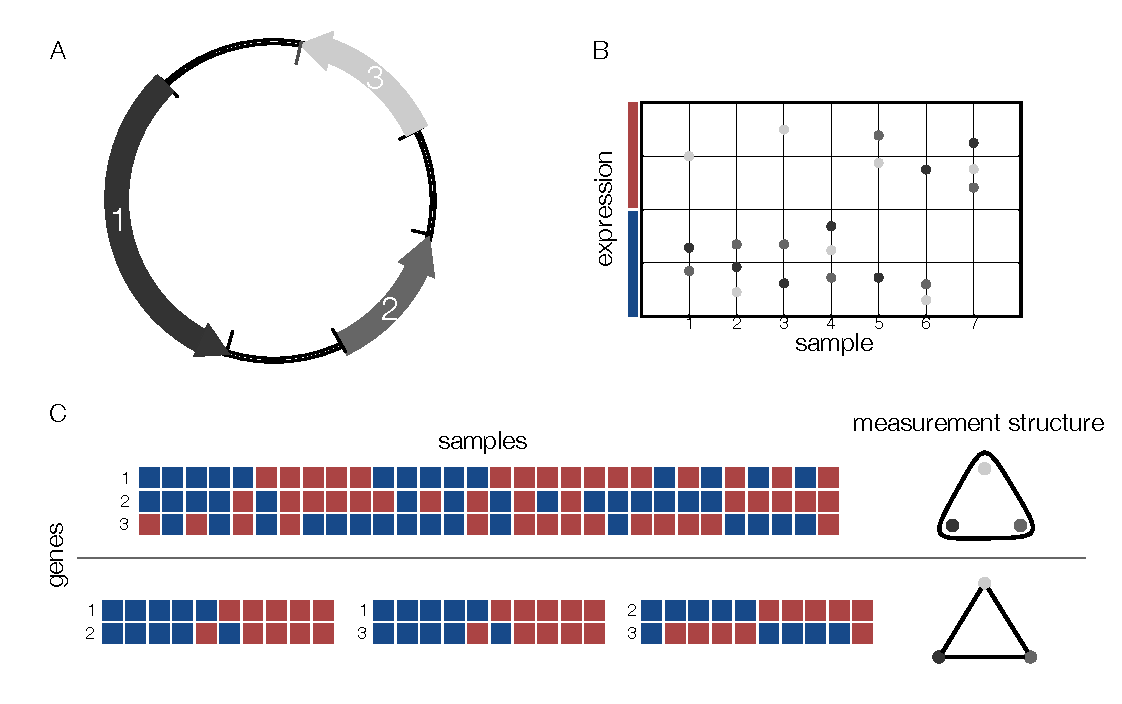
\includegraphics[width=0.9\columnwidth]{fig/figure_expression_concept.pdf}
\caption{{\bf Coarse-graining of gene expression data.}}
\label{fig:expression_concept}
\end{figure}

\begin{figure}[!ht]
\centering
\noindent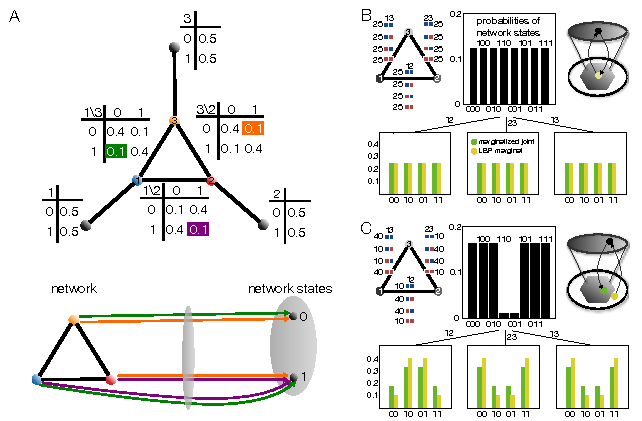
\includegraphics[width=0.9\columnwidth]{fig/inconsistentthreecycle.pdf}
\caption{{\bf Probabilistic graphical model of inconsistent gene expression data.}}
\label{fig:inconsistentthreecycle}
\end{figure}

\begin{figure}[!ht]
\centering
\noindent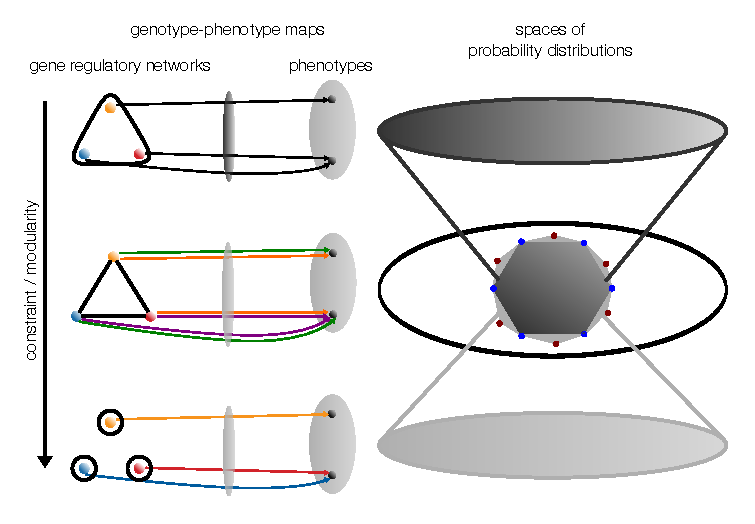
\includegraphics[width=0.9\columnwidth]{fig/conediagram.pdf}
\caption{{\bf Relationship between gene regulatory network models and spaces of probability distributions.}}
\label{fig:conediagram}
\end{figure}

\begin{figure}[!ht]
\centering
\noindent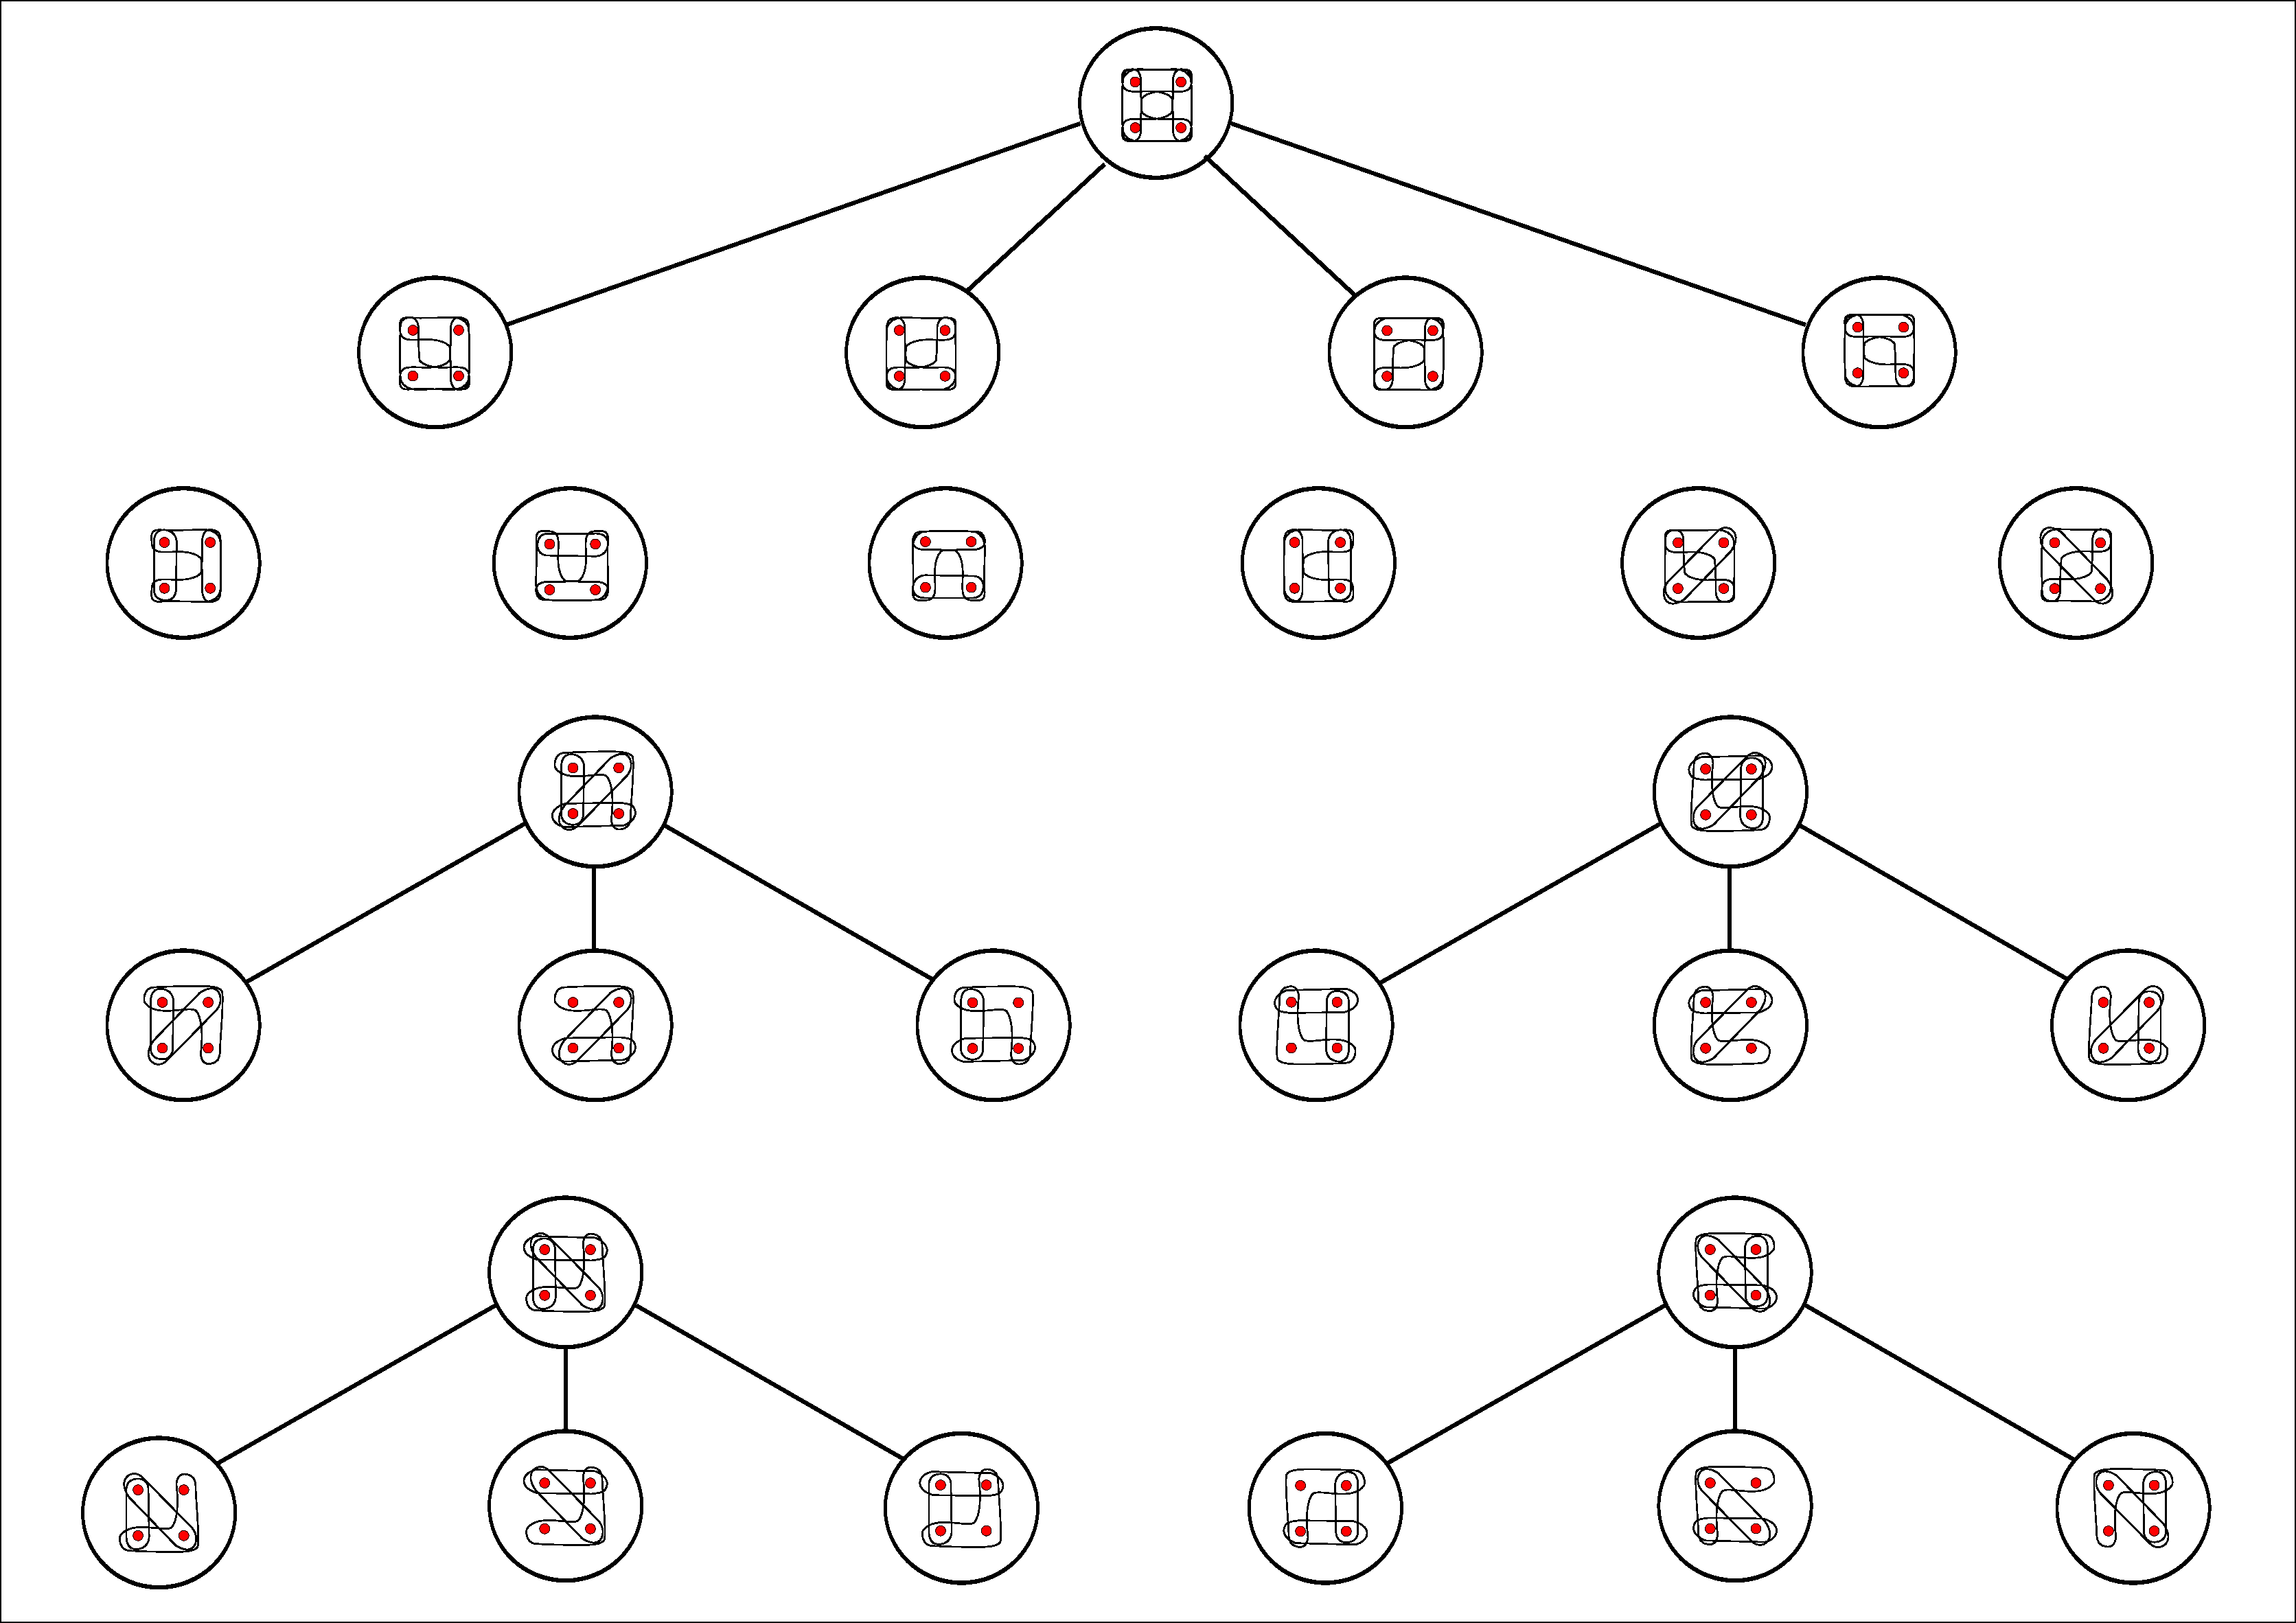
\includegraphics[width=0.9\columnwidth]{fig/non2uniformcyclichypergraphhasse.pdf}
\caption{{\bf Hierarchical relationships among all possible classes of hypergraphs that are not graphs (i.e. not 2-uniform) but have cycles.}}
\label{fig:non2uniformcyclichypergraphhasse}
\end{figure}

\begin{figure}[!ht]
\centering
\noindent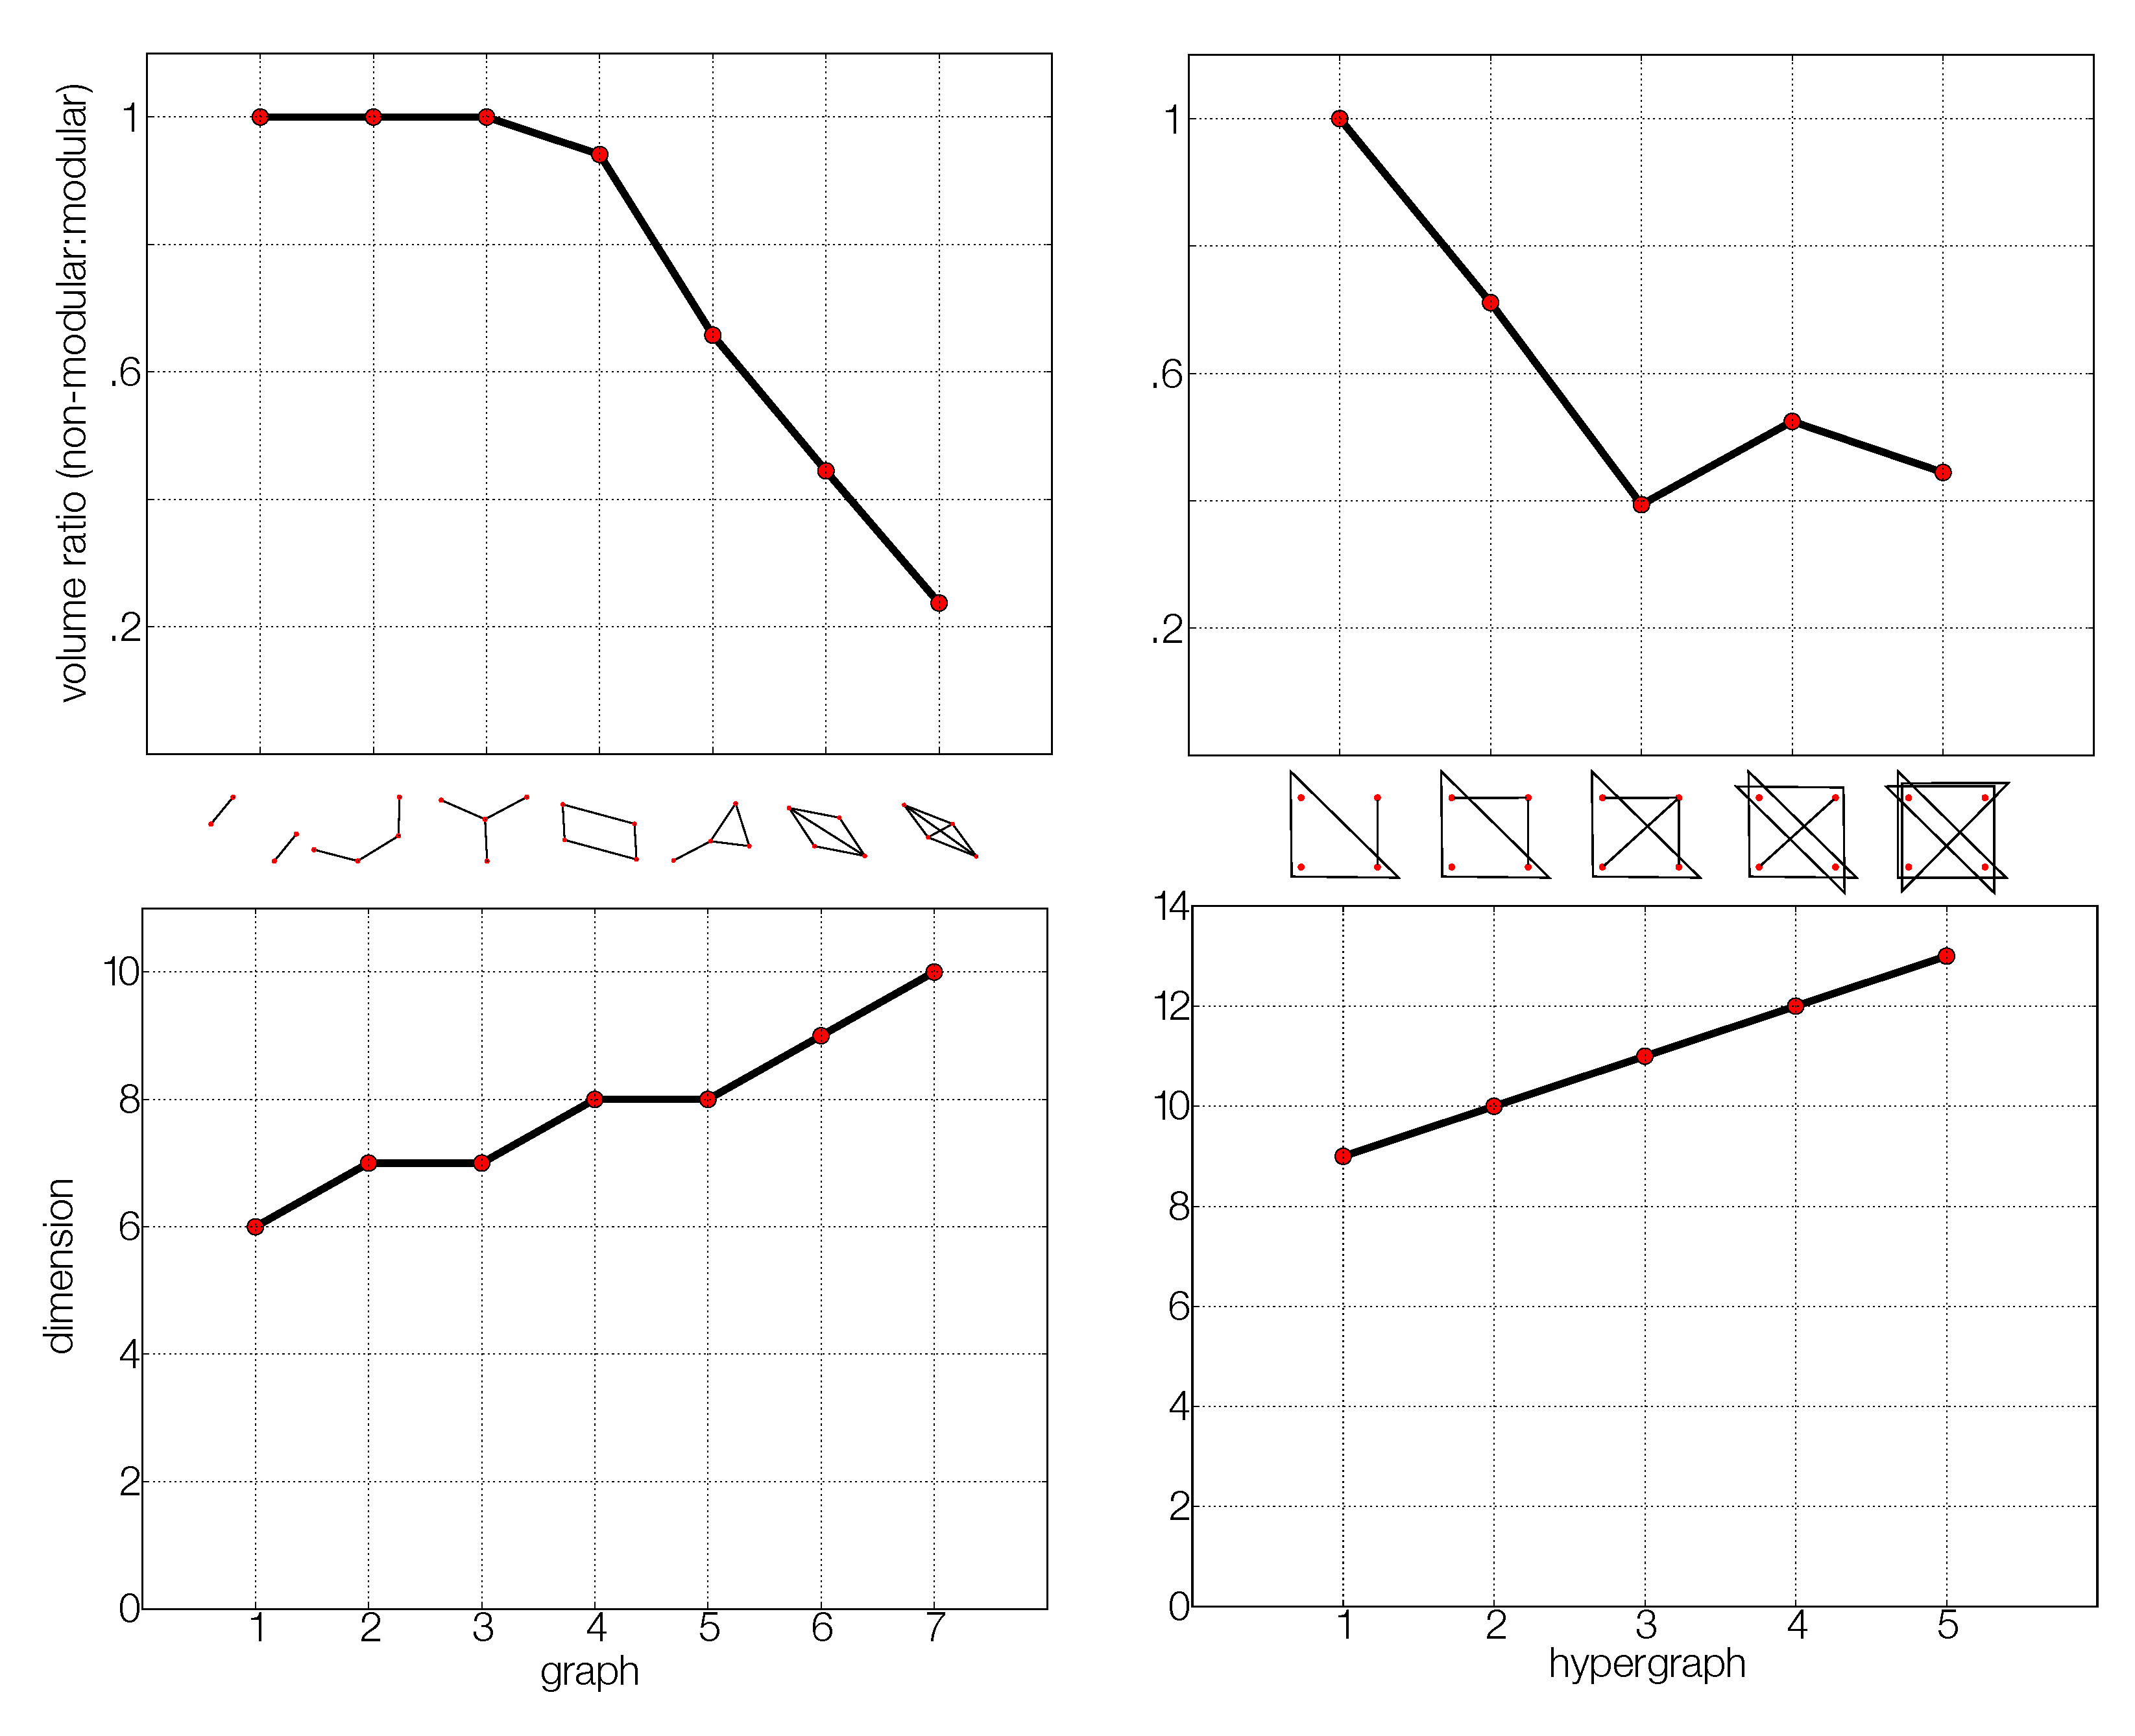
\includegraphics[width=0.9\columnwidth]{fig/figure_graphs_dims.pdf}
\caption{{\bf Non-modular to modular probability space volume ratio.}}
\label{fig:ncycvolrat}
\end{figure}

\FloatBarrier

\section*{Tables}
%\begin{table}[!ht]
%\caption{
%\bf{Table title}}
%\begin{tabular}{|c|c|c|}
%table information
%\end{tabular}
%\begin{flushleft}Table caption
%\end{flushleft}
%\label{tab:label}
% \end{table}
%!TEX root = ../plos_template.tex
\begin{table}[!ht]
\centering
\begin{tabular}{ r || c }
$l_1 l_2 l_3 l_4$ & probability \\ \hline
0000 & $q_1$ \\
0010 & $q_2$ \\
0001 & $q_3$ \\
0011 & $q_4$ \\
1000 & $q_5$ \\
1010 & $q_6$ \\
1001 & $q_7$ \\
1011 & $q_8$ \\
0100 & $q_9$ \\
0110 & $q_{10}$ \\
0101 & $q_{11}$ \\
0111 & $q_{12}$ \\
1100 & $q_{13}$ \\
1110 & $q_{14}$ \\
1101 & $q_{15}$ \\
1111 & $q_{16}$
\end{tabular}
\caption{Example of a distribution defined on the collection of maps from the set of all possible alleles, $L$, to the set of phenotype values, $P$. Such a distribution may be an instance of a global section $d \in \mathcal{D}_R\mathcal{E}(L)$ if it satisfies the sheaf condition with respect to some collection of marginal distributions. Here each row represents the probability assigned to a map in the collection of maps given by the set $P^L$. For example, $P[l_1=0,l_2=0,l_3=0,l_4=0]=q_1$ gives the probability associated to the map $\{l_1, l_2, l_3, l_4\} \mapsto \{0,0,0,0\}$.}
\label{tab:hidvarmod}
\end{table}

\begin{table}
\centering
\begin{subtable}[t]{0.4\textwidth}
\centering
\begin{tabular}{ l || c | c | c | r }
	$L_1 L_2$  &	00 & 01 & 10 & 11\\ \hline
    $l_1 l_2$ & $e_1$ & $e_2$ & $e_3$ & $e_4$\\ \hline
    $l_1 l'_2$ & $e_5$ & $e_6$ & $e_7$ & $e_8$\\ \hline
    $l'_1 l_2$ & $e_9$ & $e_{10}$ & $e_{11}$ & $e_{12}$\\ \hline
    $l'_1 l'_2$ & $e_{13}$ & $e_{14}$ & $e_{15}$ & $e_{16}$\\
    \hline
    \end{tabular}
    \caption{genotype-phenotype maps}
    \label{tab:gpm}
\end{subtable}
~~~~~~
\begin{subtable}[t]{0.4\textwidth}
\centering
	\begin{tabular}{ l || c | c | c | r }
	$L_1 L_2$  &	00 & 01 & 10 & 11\\ \hline
    $l_1 l_2$ & $p_1$ & $p_2$ & $p_3$ & $p_4$\\ \hline
    $l_1 l'_2$ & $p_5$ & $p_6$ & $p_7$ & $p_8$\\ \hline
    $l'_1 l_2$ & $p_9$ & $p_{10}$ & $p_{11}$ & $p_{12}$\\ \hline
    $l'_1 l'_2$ & $p_{13}$ & $p_{14}$ & $p_{15}$ & $p_{16}$\\
    \hline
	\end{tabular}
	\caption{probabilities}
    \label{tab:probabilities}
\end{subtable}
\caption{Genotype-phenotype mapping and associated probability tables for the two locus-two phenotype value example. We use an abbreviated notation in which we use the rewrite rules $l_1 l_2 \rightarrow \{l_1, l_2\}$ and $00 \rightarrow \{0, 0\}$ and all others analogous to avoid an excessive number of brackets.}
\label{tab:example}
\end{table}
\begin{table}[!ht]
\centering
%!TEX root = ../plos_template.tex
\begin{subtable}[t]{0.4\textwidth}
\centering
\begin{tabular}{ l || c | r }
	$L$  &	0 & 1\\ \hline
    $l_1$ & \cellcolor{DeepBlue!35} $p^*_1$ & \cellcolor{DeepRed!35} $p^*_2$\\ \hline
    $l'_1$ & $p^*_3$ & $p^*_4$\\ \hline
    $l_2$ & $p^*_5$ & $p^*_{6}$\\ \hline
    $l'_2$ & $p^*_{7}$ & $p^*_{8}$\\
    \hline
    \end{tabular}
    \caption{$l_1$}
    \label{tab:il1}
\end{subtable}
~~~~~~
\begin{subtable}[t]{0.4\textwidth}
\centering
	\begin{tabular}{ l || c | c | c | r }
	$L_1 L_2$  &	00 & 10 & 01 & 11\\ \hline
    $l_1 l_2$ & \cellcolor{DeepBlue!35} $p_1$ & \cellcolor{DeepRed!35} $p_2$ & \cellcolor{DeepBlue!35} $p_3$ & \cellcolor{DeepRed!35} $p_4$\\ \hline
    $l_1 l'_2$ & \cellcolor{DeepBlue!35} $p_5$ & \cellcolor{DeepRed!35} $p_6$ & \cellcolor{DeepBlue!35} $p_7$ & \cellcolor{DeepRed!35} $p_8$\\ \hline
    $l'_1 l_2$ & $p_9$ & $p_{10}$ & $p_{11}$ & $p_{12}$\\ \hline
    $l'_1 l'_2$ & $p_{13}$ & $p_{14}$ & $p_{15}$ & $p_{16}$\\
    \hline
	\end{tabular}
	\caption{$l_1$}
    \label{tab:dl1}
\end{subtable}

\begin{subtable}[t]{0.4\textwidth}
\centering
\begin{tabular}{ l || c | r }
	$L$  &	0 & 1\\ \hline
    $l_1$ & $p^*_1$ & $p^*_2$\\ \hline
    $l'_1$ & \cellcolor{blue!25} $p^*_3$ & \cellcolor{green!25} $p^*_4$\\ \hline
    $l_2$ & $p^*_5$ & $p^*_{6}$\\ \hline
    $l'_2$ & $p^*_{7}$ & $p^*_{8}$\\    
    \hline
    \end{tabular}
    \caption{$l_2$}
    \label{tab:il2}
\end{subtable}
~~~~~~
\begin{subtable}[t]{0.4\textwidth}
\centering
	\begin{tabular}{ l || c | c | c | r }
	$L_1 L_2$  &	00 & 01 & 10 & 11\\ \hline
    $l_1 l_2$ & $p_1$ & $p_2$ & $p_3$ & $p_4$\\ \hline
    $l_1 l'_2$ & $p_5$ & $p_6$ & $p_7$ & $p_8$\\ \hline
    $l'_1 l_2$ & \cellcolor{blue!25} $p_9$ & \cellcolor{blue!25} $p_{10}$ & \cellcolor{green!25} $p_{11}$ & \cellcolor{green!25} $p_{12}$\\ \hline
    $l'_1 l'_2$ & \cellcolor{blue!25} $p_{13}$ & \cellcolor{blue!25} $p_{14}$ & \cellcolor{green!25} $p_{15}$ & \cellcolor{green!25} $p_{16}$\\
    \hline
	\end{tabular}
	\caption{$l_2$}
    \label{tab:dl2}
\end{subtable}
%!TEX root = ../plos_template.tex
\begin{subtable}[t]{0.4\textwidth}
\centering
\begin{tabular}{ l || c | r }
	$L$  &	0 & 1\\ \hline
    $l_1$ & $p^*_1$ & $p^*_2$\\ \hline
    $l'_1$ & $p^*_3$ & $p^*_4$\\ \hline
    $l_2$ & \cellcolor{DeepBlue!35} $p^*_5$ & \cellcolor{DeepRed!35} $p^*_{6}$\\ \hline
    $l'_2$ & $p^*_{7}$ & $p^*_{8}$\\
    \hline
    \end{tabular}
    \caption{$l_3$}
    \label{tab:il3}
\end{subtable}
~~~~~~
\begin{subtable}[t]{0.4\textwidth}
\centering
	\begin{tabular}{ l || c | c | c | r }
	$L_1 L_2$  &	00 & 10 & 01 & 11\\ \hline
    $l_1 l_2$ & \cellcolor{DeepBlue!35} $p_1$ & \cellcolor{DeepBlue!35} $p_2$ & \cellcolor{DeepRed!35} $p_3$ & \cellcolor{DeepRed!35} $p_4$\\ \hline
    $l_1 l'_2$ &  $p_5$ & $p_6$ & $p_7$ & $p_8$\\ \hline
    $l'_1 l_2$ & \cellcolor{DeepBlue!35} $p_9$ & \cellcolor{DeepBlue!35} $p_{10}$ & \cellcolor{DeepRed!35} $p_{11}$ & \cellcolor{DeepRed!35} $p_{12}$\\ \hline
    $l'_1 l'_2$ & $p_{13}$ & $p_{14}$ & $p_{15}$ & $p_{16}$\\
    \hline
	\end{tabular}
	\caption{$l_3$}
    \label{tab:dl3}
\end{subtable}

%!TEX root = ../plos_template.tex
\begin{subtable}[t]{0.4\textwidth}
\centering
\begin{tabular}{ l || c | r }
	$L$  &	0 & 1\\ \hline
    $l_1$ & $p^*_1$ & $p^*_2$\\ \hline
    $l'_1$ & $p^*_3$ & $p^*_4$\\ \hline
    $l_2$ & $p^*_5$ & $p^*_{6}$\\ \hline
    $l'_2$ & \cellcolor{DeepBlue!35} $p^*_{7}$ & \cellcolor{DeepRed!35} $p^*_{8}$\\
    \hline
    \end{tabular}
    \caption{$l_4$}
    \label{tab:il4}
\end{subtable}
~~~~~~
\begin{subtable}[t]{0.4\textwidth}
\centering
	\begin{tabular}{ l || c | c | c | r }
	$L_1 L_2$  &	00 & 10 & 01 & 11\\ \hline
    $l_1 l_2$ & $p_1$ & $p_2$ & $p_3$ & $p_4$\\ \hline
    $l_1 l'_2$ & \cellcolor{DeepBlue!35} $p_5$ & \cellcolor{DeepBlue!35} $p_6$ & \cellcolor{DeepRed!35} $p_7$ & \cellcolor{DeepRed!35} $p_8$\\ \hline
    $l'_1 l_2$ & $p_9$ & $p_{10}$ & $p_{11}$ & $p_{12}$\\ \hline
    $l'_1 l'_2$ & \cellcolor{DeepBlue!35} $p_{13}$ & \cellcolor{DeepBlue!35} $p_{14}$ & \cellcolor{DeepRed!35} $p_{15}$ & \cellcolor{DeepRed!35} $p_{16}$\\
    \hline
	\end{tabular}
	\caption{$l_4$}
    \label{tab:dl4}
\end{subtable}

\caption{The sheaf condition for the two-locus-two phenotype value example. The left column represents \emph{atomic} probabilities that relate probabilities via equations \ref{eq:pparsys} from the empirical models given in the right hand column. Each row in all tables is required to sum to 1.}
\label{tab:sheaf}
\end{table}

\begin{table}[!ht]
\centering
\begin{tabular}{ c | l | c }
	\textbf{notation} & \textbf{description} & \textbf{size}\\ \hline \hline
	$\{l_1,l_2\}$ & set of genetic loci & $g = 2$\\ \hline
	$\{a_1,a_2\}$ & set of distinct alleles available to each locus & $a = 2$\\ \hline
	$\{0,1\}$ & set of phenotype values & $p = 2$\\ \hline
	$\{(0,0),(0,1),(1,0),(1,1)\}$ & set of phenotype assignments & $p^g = 4$\\ \hline
	$L = \{l_1,l_2,l'_1,l'_2\}$ & set of all possible alleles for all loci & $ga = 4$\\ \hline
	$\{l_1 l_2,l'_1 l_2,l_1 l'_2,l'_1 l'_2\}$ & set of gene regulatory network modules & $a^g = 4$\\ \hline
$\coprod_{O \in \mathcal{G}} \mathcal{E}(O)$ & set of modularized genotype-phenotype maps  & $(ap)^g = 16$\\ \hline
	$\mathcal{E}(L) = P^L$ & set of global genotype-phenotype maps & $p^{ga} = 16$\\
    \end{tabular}
\caption{Summary of concrete parameter values $(g,a,p)$ in terms of abstract notation for $(g=2,a=2,p=2)$. Note that $\{l_1,l_2,l'_1,l'_2\} \equiv \{l_1,l_2\} \times \{a_1,a_2\}$.}
\label{tab:pars222}
\end{table}

%!TEX root = ../plos_template.tex
\begin{table}[!ht]
\centering
\begin{tabular}{ r || c | c | c | c | c | c | c | c | c | c | c | c | c | c | c | c }
		 &	\begin{sideways}$e^{1234}_{0000}$\end{sideways} & \begin{sideways}$e^{1234}_{0010}$\end{sideways} & \begin{sideways}$e^{1234}_{0001}$\end{sideways} & \begin{sideways}$e^{1234}_{0011}$\end{sideways}
			  & \begin{sideways}$e^{1234}_{1000}$\end{sideways} & \begin{sideways}$e^{1234}_{1010}$\end{sideways} & \begin{sideways}$e^{1234}_{1001}$\end{sideways} & \begin{sideways}$e^{1234}_{1011}$\end{sideways}
			  &	\begin{sideways}$e^{1234}_{0100}$\end{sideways} & \begin{sideways}$e^{1234}_{0110}$\end{sideways} & \begin{sideways}$e^{1234}_{0101}$\end{sideways} & \begin{sideways}$e^{1234}_{0111}$\end{sideways}
			  &	\begin{sideways}$e^{1234}_{1100}$\end{sideways} & \begin{sideways}$e^{1234}_{1110}$\end{sideways} & \begin{sideways}$e^{1234}_{1101}$\end{sideways} & \begin{sideways}$e^{1234}_{1111}$\end{sideways}\\ \hline \hline
    $e^{12}_{00}$ & 1 & 1 & 1 & 1 & 0 & 0 & 0 & 0 & 0 & 0 & 0 & 0 & 0 & 0 & 0 & 0\\ \hline
    $e^{12}_{10}$ & 0 & 0 & 0 & 0 & 1 & 1 & 1 & 1 & 0 & 0 & 0 & 0 & 0 & 0 & 0 & 0\\ \hline
    $e^{12}_{01}$ & 0 & 0 & 0 & 0 & 0 & 0 & 0 & 0 & 1 & 1 & 1 & 1 &  0 & 0 & 0 & 0\\ \hline
    $e^{12}_{11}$ & 0 & 0 & 0 & 0 & 0 & 0 & 0 & 0 & 0 & 0 & 0 & 0 & 1 & 1 & 1 & 1\\ \hline

    $e^{32}_{00}$ & 1 & 0 & 1 & 0 & 1 & 0 & 1 & 0 & 0 & 0 & 0 & 0 & 0 & 0 & 0 & 0\\ \hline
    $e^{32}_{10}$ & 0 & 1 & 0 & 1 & 0 & 1 & 0 & 1 & 0 & 0 & 0 & 0 & 0 & 0 & 0 & 0\\ \hline
    $e^{32}_{01}$ & 0 & 0 & 0 & 0 & 0 & 0 & 0 & 0 & 1 & 0 & 1 & 0 & 1 & 0 & 1 & 0\\ \hline
    $e^{32}_{11}$ & 0 & 0 & 0 & 0 & 0 & 0 & 0 & 0 & 0 & 1 & 0 & 1 & 0 & 1 & 0 & 1\\ \hline

    $e^{14}_{00}$ & 1 & 1 & 0 & 0 & 0 & 0 & 0 & 0 & 1 & 1 & 0 & 0 & 0 & 0 & 0 & 0\\ \hline
    $e^{14}_{10}$ & 0 & 0 & 0 & 0 & 1 & 1 & 0 & 0 & 0 & 0 & 0 & 0 & 1 & 1 & 0 & 0\\ \hline
    $e^{14}_{01}$ & 0 & 0 & 1 & 1 & 0 & 0 & 0 & 0 & 0 & 0 & 1 & 1 & 0 & 0 & 0 & 0\\ \hline
    $e^{14}_{11}$ & 0 & 0 & 0 & 0 & 0 & 0 & 1 & 1 & 0 & 0 & 0 & 0 & 0 & 0 & 1 & 1\\ \hline

    $e^{34}_{00}$ & 1 & 0 & 0 & 0 & 1 & 0 & 0 & 0 & 1 & 0 & 0 & 0 & 1 & 0 & 0 & 0\\ \hline
    $e^{34}_{10}$ & 0 & 1 & 0 & 0 & 0 & 1 & 0 & 0 & 0 & 1 & 0 & 0 & 0 & 1 & 0 & 0\\ \hline
    $e^{34}_{01}$ & 0 & 0 & 1 & 0 & 0 & 0 & 1 & 0 & 0 & 0 & 1 & 0 & 0 & 0 & 1 & 0\\ \hline
    $e^{34}_{11}$ & 0 & 0 & 0 & 1 & 0 & 0 & 0 & 1 & 0 & 0 & 0 & 1 & 0 & 0 & 0 & 1\\
    \end{tabular}
\caption{Explicit construction of $\mathbf{G}_{n \times m}$ for the case $L = \{ l_1,l_2,l_3,l_4 \}$, $\mathcal{G} = \{\{l_1,l_2 \},\{l_1,l_4 \},\{l_3,l_2\},\{l_3,l_4\} \}$, $P=\{0,1\}$ and thus $\mathbf{G}_{(2 \cdot 2)^2 \times 2^{2 \cdot 2}} = \mathbf{G}_{16 \times 16}$.}
\label{tab:logmat222}
\end{table}


\FloatBarrier

\section*{Polymake computation of the non-modular:modular volume ratio of probability distribution polytopes for cyclic hypergraphs on three and four vertices}
%!TEX root = ../plos_template.tex
\begin{python}
"""
hypergraphvolrat.py

given a hypergraph generate a minimal / full-dimensional representation
of the inequalities definitive of (H-rep) the locally consistent
polytope of probability distributions and compute the ratio of its
volume to that of the corresponding globally consistent polytope
"""
import sys
import numpy as np
import sympy as sp
import subprocess
import re
import itertools
from fractions import Fraction

from graphlist4 import graphdict

def kcfromgraph(edgelist=[(0,1),(1,2),(2,3),(3,0)],
                graphname="graph", pvallist=None,
                printlevel=1):
    """
    input: edgelist = the list of edges of a graph
           pvallength = the number of discrete values each node can take
    output: polrepindineqs - polymake compatible minimal
                              representation
            poldim - expected dimension of the resulting polytope
    """
    maxcliques = map(list, edgelist)

    numnodes = len(set([item for sublist in maxcliques for item in sublist]))

    if pvallist is None:
        pvallist = 2*np.ones(numnodes,dtype=np.int)

    stateindices = itertools.product(*map(range,pvallist))
    columns_states = [list(element) for element in stateindices]

    cliquevals = []
    cliqueids = []
    for clique in maxcliques:
        cliquevaliter = itertools.product(*map(range,
                                         [pvallist[i] for i in clique]))
        for cliqueval in cliquevaliter:
            cliquevals.append(list(cliqueval))
            cliqueids.append(clique)

    normconds = np.zeros((len(maxcliques),len(cliqueids)),dtype=np.int)
    normconds = np.append(normconds, np.ones_like(normconds[:,0])[...,None],1)
    for i,maxclique in enumerate(maxcliques):
        for j,cliqueid in enumerate(cliqueids):
            if maxclique==cliqueid:
                normconds[i,j]=1

    ssmat = np.zeros((len(cliquevals),
                      len(columns_states)),dtype=int)

    for i,(cv,cid) in enumerate(zip(cliquevals,cliqueids)):
        for j,cs in enumerate(columns_states):
            if cv==[cs[k] for k in cid]:
                ssmat[i,j]=1

    # Read ssmat from macaulay file
    # fname = '../macaulay/C4_bin.mat'
    # with open(fname) as f:
    #     next(f)
    #     ssmat = np.array([ map(int,line.split()) for line in f ])

    eqmat = np.asarray(sp.Matrix(ssmat.T).nullspace(simplified=True),
                       dtype=np.int)
    eqmat = np.append(eqmat, np.zeros_like(eqmat[:,0])[...,None],1)
    eqmat = np.vstack((eqmat, normconds))

    kceqsref, ind = sp.Matrix(eqmat).rref(simplified=True)
    kceqsrefs = np.squeeze(np.asarray(kceqsref))
    kceqsrefa = kceqsrefs[~np.all(kceqsrefs == 0, axis=1)]

    im1 = np.arange(kceqsrefa.shape[1])
    mask1 = np.ones(len(im1), dtype=bool)
    mask1[ind] = False

    indineqs = kceqsrefa[:, im1[mask1]]

    polrepindineqs = np.zeros(shape=np.shape(indineqs), dtype=np.int)
    polrepindineqs[:, 1:] = -1*indineqs[:, :-1]
    polrepindineqs[:, 0] = indineqs[:, -1]

    poldim = polrepindineqs.shape[1] - 1

    if printlevel:
        print "KC / sufficient statistics matrix"
        print ssmat
        print ""

        print "Full set of equalities (non-homogeneous rhs for normalization)"
        print eqmat
        print ""

        print "Reduced equalities (non-homogeneous rhs)"
        print kceqsrefa
        print ""

        print "Polymake reduced inequalities (homogeneous rhs in first column)"
        print "Each line describes one linear inequality."
        print "The encoding is as follows: "
        print "(a_0,a_1,...,a_d) is the inequality"
              "a_0 + a_1 x_1 + ... + a_d x_d >= 0."
        print polrepindineqs
        print ""

        print "dimension %d\n" % poldim

    return polrepindineqs, poldim

def bmatrix(a):
    """Returns a LaTeX bmatrix

    :a: numpy array
    :returns: LaTeX bmatrix as a string
    """
    if isinstance(a, np.ndarray):
        if len(a.shape) > 2:
            raise ValueError('bmatrix can at most display two dimensions')
        lines = str(a).replace('[', '').replace(']', '').splitlines()
    elif isinstance(a, str):
        lines = a.splitlines()
    else:
        raise ValueError('wrong input type')
    rv = [r'\begin{bmatrix}']
    rv += ['  ' + ' & '.join(l.split()) + r'\\' for l in lines]
    rv +=  [r'\end{bmatrix}']
    return '\n'.join(rv)

def posineqgen(poldim):
    """
    output: polymake compatibile positivity inequalities
    """
    posineq = np.zeros(shape=(poldim, poldim+1), dtype=np.int)
    posineq[:, 1:] = np.identity(poldim)
    return posineq

def minineqgen(eqfname):
    """
    output: minineqs - combine the Kolmogorov Consistency inequalities
                       with positivity inequalities
    """
    eqmat, poldim = kcfromgraph(graphdict[eqfname],eqfname)
    posmat = posineqgen(poldim)
    minineqs = eqmat.tolist() + posmat.tolist()

    return minineqs, poldim

def runpolymakescript(minineqs, representation, polyproperty, eqfname='graph'):
    """
    intermediate: filestring - polymake script with full-dimensional / minimal
                         H-representation of the Kolmogorov Consistent
                         polytope
    output: polyout - output of polymake for given minineqs and
                      polyproperty
    """
    filestring = str("$Verbose::credits=0;\nuse application "
                     "\"polytope\";\nmy $ndineqs=new "
                     "Matrix<Rational>(%s);\nmy $nd=new "
                     "Polytope<Rational>(%s=>$ndineqs);\nprint "
                     "$nd->%s;" %
                     (str(minineqs), representation, polyproperty))

    scriptname = eqfname + "kcscript.pl"
    fname = open(scriptname,'w')
    fname.write(filestring)
    fname.close()
    polyout = subprocess.check_output(["polymake", "--script",
                                               scriptname])

    return polyout

def booleverts(polyvertices):
    """
    remove rational vertices
    """
    def filtrat(line):
        """
        filter lines with '/'s indicating rational numbers
        """
        if "/" not in line:
            vert = [int(x) for x in line.split(' ')]
            return vert
        else:
            return

    filtverts = [filtrat(line)
                             for line in polyvertices.split('\n')[:-1]]
    filtverts = [l for l in filtverts if l is not None]
    return filtverts

def convert(srat):
    """
    convert rational number string to float
    """
    try:
        return float(srat)
    except ValueError:
        num, denom = srat.split('/')
        return float(num) / float(denom)

def approxvol(minineqs,eqfname,error_threshold=0.2):
    minineqstr = re.sub(r'], ',r'],\n',str(minineqs))

    centroid = list(0.125*np.ones(np.shape(minineqs)[1]-1))
    filestring = str("addpath('volconvbod');\n"
                     "aa=%s;\n"
                     "bb = [aa(:,2:end) aa(:,1)];\n"
                     "bb(:,1:end-1)=-1*bb(:,1:end-1);\n"
                     "intpoint = %s';\n"
                     "Volume(bb,[],%s,intpoint)" %
                     (minineqstr, centroid, error_threshold))
    scriptname = eqfname + "Vol"
    fname = open(scriptname + ".m",'w')
    fname.write(filestring)
    fname.close()

    #matlab -nodesktop -nojvm -nosplash -r "run polymakeVol; exit;"
    matprocout = subprocess.check_output(["matlab", "-nodesktop",
                                      "-nojvm", "-nosplash",
                                      "-logfile", scriptname + ".out",
                                      "-r", scriptname + "; exit;"])
    fname = open(scriptname + ".out")
    matout = fname.read()
    fname.close()
    vollist = re.findall(r'(?<=Final Volume: ).*(?=,)',matout)
    vol = float(vollist[0])
    return vol

def minineqrep(argv):
    """
    usage: python minineqrep.py C4 VERTICES
    """
    eqfname = str(argv[0])
    polyproperty = str(argv[1])

    print "Name of graph: \n%s\n" % eqfname

    minineqs, dim = minineqgen(eqfname)
    polyout = runpolymakescript(minineqs, "INEQUALITIES",
                                polyproperty, eqfname)

    #poutbmatrix = bmatrix(polyout)

    if polyproperty == "VERTICES":
        boolepolyverts = booleverts(polyout)
        volboole = runpolymakescript(boolepolyverts,
                            "POINTS", "VOLUME", eqfname)

        volkolmogorov = runpolymakescript(minineqs,
                                        "INEQUALITIES", "VOLUME", eqfname)
        vrat = convert(volboole) / convert(volkolmogorov)
        #print "%s/%s ~ %0.6f" % (volboole, volkolmogorov, vrat)
        print "Volume of Boole polytope"
        print volboole
        print ""

        print "Volume of Kolmogorov polytope"
        print volkolmogorov
        print ""

        print "Volume ratio Boole:Kolmogorov"
        print vrat
        print ""

    print "Vertices of Kolmogorov polytope\n" + polyout
    return vrat, dim

if __name__ == "__main__":
    minineqrep(sys.argv[1:])
\end{python}

\pagebreak

\section*{Example graphs on four vertices}
%!TEX root = ../plos_template.tex
\begin{python}
"""
A subset of the non-isomorphic graphs on 4 nodes

enumerate non-isomorphic graphs
on 4 vertices
https://oeis.org/A000088/a000088a.gif
http://www.graphclasses.org/smallgraphs.html#nodes4
"""

#---------------------------------
# Binary graphs
#---------------------------------

# 2K2 = \bar{C4}
twok2 = [(0,1),(2,3)]

# claw = K_{1,3}
claw = [(0,1),(0,2),(0,3)]

# P4 = 4-chain
P4 = [(0,1),(1,2),(2,3)]

# C4 = K_{2,2}
C4 = [(0,1),(1,2),(2,3),(3,0)]

# paw = 3-pan
paw = [(0,3),(1,2),(1,3),(2,3)]

# diamond = K4 - e = 2-fan
diamond = [(0,2),(0,3),(1,2),(1,3),(2,3)]

# K4 = W3
K4 = [(0,1),(0,2),(0,3),(1,2),(2,3),(1,3)]

# C3
C3 = [(0,1),(1,2),(0,2)]

#---------------------------------
# Hypergraphs
#---------------------------------

# flagpole
flagpole = [(0,2,3),(1,2)]

# basket
basket = [(0,2,3),(0,1),(2,1)]

# tripod
tripod = [(0,2,3),(0,1),(1,2),(1,3)]

# overtwo
overtwo = [(0,1,2),(0,2,3)]

# overtwoconnect
overtwoconnect = [(0,1,2),(0,2,3),(1,3)]

# overthree
overthree = [(0,1,2),(0,1,3),(0,2,3)]

# overfour
overfour = [(0,1,2),(0,1,3),(0,2,3),(1,2,3)]

graphdict = locals()

graphlist = [twok2,
             claw,
             P4,
             C4,
             paw,
             diamond,
             K4]

hgraphlist = [flagpole,
              overtwo,
              basket,
              tripod,
              overtwoconnect,
              overthree,
              overfour]

\end{python}

\pagebreak

\section*{Generate hypergraph lattice}
\begin{python}
"""
hypergraphlattice.py

1. given a number of vertices generate a Hasse diagram
of the lattice of hypergraphs over the given number of vertices
2. use [Graham reduction](https://en.wikipedia.org/wiki/Hypergraph#Acyclicity)
to detect cycles in each hypergraph and generate a Hasse diagram of all
hypergraphs on a given number of vertices in which each hypergraph
contains at least one cycle

uses the python-lattice 0.0.2 package
https://pypi.python.org/pypi/python-lattice

uses the python dot2tex 2.8.7 package
https://pypi.python.org/pypi/dot2tex
"""

from lattice import Lattice
import itrecipes
import subprocess
import re
import dot2tex

from hypergraphcycle import testcycle

def subsetsize(ss):
    if not map(len,ss):
        return 0
    else:
        return max(map(len,ss))

def removesubsets(ss):
    fs = frozenset([m for i,m in enumerate(ss)
                    if not any(m < n for n in ss)])
    return fs

def Hasse2(L):
        graph=dict()
        for indexS,elementS in enumerate(L.Uelements):
            graph[indexS]=[]
            supersets = [(indexD,elementD)
                           for indexD,elementD in enumerate(L.Uelements)
                           if L.wrap(elementS) <= L.wrap(elementD)]
            supersets.remove((indexS,elementS))
            coverindexlist = [ind for ind,cover in supersets
                            if not any(L.wrap(cover) >= L.wrap(ostcover)
                      for i,ostcover in supersets if ostcover != cover)]
            graph[indexS]=coverindexlist
        dotcode='digraph G {\nsplines="line"\nrankdir=BT\n'
        dotcode+='\"'+str(L.TopElement.unwrap)+'\" [shape=box];\n'
        dotcode+='\"'+str(L.BottonElement.unwrap)+'\" [shape=box];\n'
        for s, ds in graph.iteritems():
            for d in ds:
                dotcode += "\""+str(L.WElementByIndex(s))+"\""
                dotcode += " -> "
                dotcode += "\""+str(L.WElementByIndex(d))+"\""
                dotcode += ";\n"
        dotcode += "}"
        try:
            from scapy.all import do_graph
            do_graph(dotcode)
        except:
            pass
        return dotcode

def Hasse3(L):
        graph=dict()
        for indexS,elementS in enumerate(L):
            graph[indexS]=[]
            supersets = [(indexD,elementD)
                           for indexD,elementD in enumerate(L)
                           if elementS <= elementD]
            supersets.remove((indexS,elementS))
            coverindexlist = [ind for ind,cover in supersets
                            if not any(cover >= ostcover
                      for i,ostcover in supersets if ostcover != cover)]
            graph[indexS]=coverindexlist

        vals = [val for k,v in graph.iteritems() for val in v]
        nakedkeys = [k for k,v in graph.iteritems() if not v]
        noionodes = [nk for nk in nakedkeys if nk not in vals]

        dotcode='digraph G {\nsplines="line"\nrankdir=BT\n'
        for g in noionodes:
            dotcode+='\"'+str(L[g])+'\" [shape=box];\n'
        #dotcode+='\"'+str(L.TopElement.unwrap)+'\" [shape=box];\n'
        #dotcode+='\"'+str(L.BottonElement.unwrap)+'\" [shape=box];\n'
        for s, ds in graph.iteritems():
            for d in ds:
                dotcode += "\""+str(L[s])+"\""
                dotcode += " -> "
                dotcode += "\""+str(L[d])+"\""
                dotcode += ";\n"
        dotcode += "}"
        # try:
        #     from scapy.all import do_graph
        #     do_graph(dotcode)
        # except:
        #     pass
        return dotcode

def genhypergraphs(vertices):
    #vertices=[1,2,3]
    #baseset = [frozenset([i]) for i in range(vertices)]
    baseset = vertices
    ps = itrecipes.powerset(baseset)
    ps.next() # burn the empty list
    psl = map(frozenset,ps)
    hg = itrecipes.powerset(psl)
    hgs = map(frozenset,hg)
    hgf = map(removesubsets,hgs)
    hgf = list(set(hgf))
    return hgf

def filteracyclic(hgraphlist, numverts):
    return [hh for hh in hgraphlist if testcycle(hh,numverts)]

def genhypergraphlattice(vertices):
    def intersection(a,b): return removesubsets(a&b)
    def union(a,b): return removesubsets(a|b)
    hgs = genhypergraphs(vertices)
    hgs = sorted(hgs,key=subsetsize)
    L = Lattice(hgs,union,intersection)
    return L

def genhypergraphhasse(L):
    #dotstring = Hasse2(L) #L.Hasse()
    dotstring = Hasse3(L)
    dotstring = dotstring.replace("set","")
    dotstring = dotstring.replace("frozen","")
    dotstring = dotstring.replace("(","")
    dotstring = dotstring.replace(")","")
    dotstring = dotstring.replace("[","{")
    dotstring = dotstring.replace("]","}")
    dotstring = re.sub(r"\{\{(?=[0-9])","{",dotstring)
    dotstring = re.sub(r"(?<=[0-9])\}\}","}",dotstring)
    print dotstring
    return dotstring

def savedotfile(vertices):
    fh = open("output/hypergraphhasse.dot","w")
    #L = genhypergraphlattice(vertices)
    #dotstring = genhypergraphhasse(L)
    ghc=genhypergraphs([1,2,3,4])
    chg = filteracyclic(ghc,4)
    dotstring = genhypergraphhasse(chg)

    fh.write("%s" % dotstring)
    fh.close()

    texcode = dot2tex.dot2tex(dotstring, format='tikz', crop=True)
    texcode = re.sub(r"\{\}","empty",texcode) # using node name {}
                                              # produces a latex error
    fh = open("output/hypergraphhasse.tex","w")
    fh.write("%s" % texcode)
    fh.close()

    subprocess.call("cd output && latexmk -pdf hypergraphhasse.tex",shell=True)
    subprocess.call("cd output && rm hypergraphhasse.log \
                        hypergraphhasse.fdb_latexmk \
                        hypergraphhasse.fls \
                        hypergraphhasse.aux",shell=True)
    subprocess.call("evince output/hypergraphhasse.pdf &",shell=True)
    subprocess.call("pdf2svg output/hypergraphhasse.pdf \
                             output/hypergraphhasse.svg",shell=True)

    # subprocess.call("dot -Tps output/hypergraphhasse.dot -o
    # output/hypergraphhasse.ps",shell=True)
    # subprocess.call("epstopdf output/hypergraphhasse.ps",shell=True)
    # subprocess.call("evince output/hypergraphhasse.pdf",shell=True)
    return dotstring
\end{python}

\pagebreak

\section*{Filter hypergraphs with cycles using Graham reduction}
\begin{python}
"""
hypergraphcycle.py

implementation of the Graham reduction method
for hypergraph cycle detection
http://web.cecs.pdx.edu/~maier/TheoryBook/MAIER/C13.pdf
"""

from copy import deepcopy
import numpy as np
import hypergraph as hg
import hypergraph.core as hgc

def remove_ear(G):
    H = deepcopy(G)
    for v in H.vertices:
        if len(H.incident(v))==1:
            edge_containing_ear = H.incident(v).pop()
            non_ear_vertices = set.difference(set(edge_containing_ear),
                                              set([v]))
            if non_ear_vertices:
                edge_lacking_ear = hgc.Edge(non_ear_vertices)
                edges_lacking_ear = deepcopy(H.edges)
                edges_lacking_ear.remove(edge_containing_ear)
                if any([edge_lacking_ear.issubset(e) for e in edges_lacking_ear]):
                    H.remove_vertex(v)
                else:
                    H.remove_edge(edge_containing_ear)
                    H.add_edge(edge_lacking_ear)
            else:
                H.remove_edge(edge_containing_ear)
            break
    return H

def graham_reduce(G):
    progress_flag = True
    cycle_flag = True
    vertex_counter = 1
    hgstack = [G]
    while progress_flag:
        H = hgstack.pop()
        temp=remove_ear(H)
        if temp.edges:
            if temp==H:
                if vertex_counter > len(G.vertices):
                    progress_flag = False
                    cycle_flag = True
            hgstack.append(temp)
        else:
            progress_flag = False
            cycle_flag = False
        vertex_counter += 1
    return cycle_flag

def testcycle(edgelist,numverts):
    hh=hgc.Hypergraph(vertices=set(range(numverts)))
    for e in edgelist:
        hh.add_edge(hgc.Edge(e))
    return graham_reduce(hh)


# for g in graphlist:
#     #print testcycle(g)
#     hh=hgc.Hypergraph(vertices=set([0,1,2,3]))
#     for e in g:
#         hh.add_edge(hgc.Edge(e))
#     print graham_reduce(hh)
\end{python}

\pagebreak

\section*{Approximate volume computations}
\begin{python}
"""
overfourapproxvol.py

use

B. Cousins and S. Vempala, A Cubic Algorithm for Computing Gaussian Volume.
2013. [arXiv:1306.5829](http://arxiv.org/abs/1306.5829v2).

to approximate the volume of the globally consistent polytope
for the case of the overfour graph

overfour = [(0,1,2),(0,1,3),(0,2,3),(1,2,3)]
"""

from minineqrep import *

def approxvol(minineqs,eqfname,error_threshold=0.2):
    minineqstr = re.sub(r'], ',r'],\n',str(minineqs))
    #polyout = runpolymakescript(minineqs,
    #                        "INEQUALITIES", "CENTROID", eqfname)
    #centroid = [float(Fraction(s)) for s in polyout.split()][1:]
    centroid = list(0.125*np.ones(np.shape(minineqs)[1]-1))
    filestring = str("addpath('volconvbod');\n"
                     "aa=%s;\n"
                     "bb = [aa(:,2:end) aa(:,1)];\n"
                     "bb(:,1:end-1)=-1*bb(:,1:end-1);\n"
                     "intpoint = %s';\n"
                     "Volume(bb,[],%s,intpoint)" %
                     (minineqstr, centroid, error_threshold))
    scriptname = eqfname + "Vol"
    fname = open(scriptname + ".m",'w')
    fname.write(filestring)
    fname.close()
    #matlab -nodesktop -nojvm -nosplash -r "run polymakeVol; exit;"
    matprocout = subprocess.check_output(["matlab", "-nodesktop",
                                      "-nojvm", "-nosplash",
                                      "-logfile", scriptname + ".out",
                                      "-r", scriptname + "; exit;"])
    fname = open(scriptname + ".out")
    matout = fname.read()
    fname.close()
    vollist = re.findall(r'(?<=Final Volume: ).*(?=,)',matout)
    vol = float(vollist[0])
    return vol

eqfname = "overfour"
minineqs,dim=minineqgen("overfour")
polyout = runpolymakescript(minineqs, "INEQUALITIES", "VERTICES", "overfour")
boolepolyverts = booleverts(polyout)
volboole = runpolymakescript(boolepolyverts,
                            "POINTS", "VOLUME", eqfname)
volkc = approxvol(minineqs,"overfour",0.01)

#9.17659647818378e-11/3.877906e-10
vol = convert(volboole)/volkc
\end{python}


\end{document}
